\subsection{Primäre Energieskalen}

\begin{fquestion}{Energieeigenwerte im Wasserstoffatom?}
    $E_n = \frac{E_R}{n^2}$ mit Rydberg-Energie $E_R = \alpha^2  \frac{\mu}{2} = 13.6\,$eV.
\end{fquestion}

\begin{fquestion}{Wie ist die Feinstrukturkonstante definiert? }
    $\alpha = \frac{e^2}{4\pi\epsilon_0\hbar c} \approx \frac{1}{137}$
\end{fquestion}

\begin{fquestion}{Ohne Feinstruktur, was gibt es noch für Niveaus?}
    Ohne Feinstruktur ist die Energie noch unabhängig von der Drehimpulsquantenzahl $l$.
    Selbst mit Feinstruktur ist die Energie aber unabhängig von der $z$-Komponente, also der Quantenzahl $m = -l, \dots , l$.
    Das muss auch so sein, weil $m$ lediglich die Projektion von $\Vec{L}$ auf eine willkürlich gewählt Achse (hier die $z$-Achse) beschreibt.
    Die Skizze dieser Projektion 
    \begin{center}
        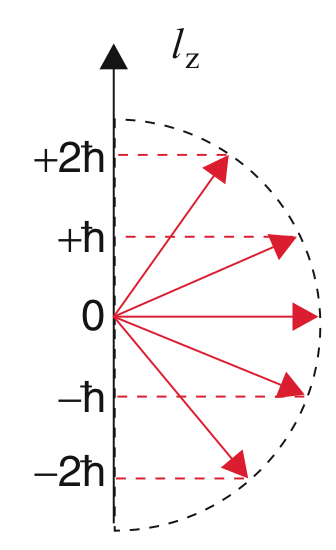
\includegraphics[width=0.25\linewidth]{img/Projektion_Magnetquantenzahl.png}
    \end{center}
    Abbildung unverändert aus ``Demtröder: Experimentalphysik 3 -- Atome, Moleküle und Festkörper, S. 151''. 
    \\
    Das ist auch für beliebige andere Zentralpotentiale der Fall.
    Mathematisch kann man auch über den Separationsansatz argumentieren, da $m$ nicht in der Radialgleichung auftaucht, und damit die Energie nicht beeinflussen kann.
\end{fquestion}

\begin{fquestion}{Wie kann man grob Grundzustand und Bindungsradius abschätzen?}
    Heisenberg-Unschärfe, z.B. $\Delta x \Delta p \simeq \hbar$.
    Daraus folgt $\Delta p \simeq \frac{1}{\Delta x}$ und $r_0 \simeq \frac{1}{p_0}$.
    Dabei ist $E_\text{kin} = \frac{p_0^2}{2\mu} \simeq \frac{1}{2\mu r_0^2}$.
    Für das Coulomb-Potential ist
    $$E = E_\text{kin} + E_\text{pot} = \frac{1}{2\mu r^2} - \frac{\alpha}{r},$$
    wobei das Minimum durch $0 = -\frac{1}{\mu r_0^3} + \frac{\alpha}{r_0^2}$, also $r_0 = \frac{1}{\mu\alpha} $, gegeben ist.
    Die Grundzustandsenergie ist damit etwa $E_0 \simeq \frac{1}{2\mu r_0^2} = \alpha^2\frac{\mu }{2}$.
\end{fquestion}

\begin{fquestion}{Was sind die Quantenzahlen bei Wasserstoff?}
    Hauptquantenzahl $n$, (Bahn-)Drehimpulsquantenzahl $l$, magnetische Quantenzahl $m$ (oder auch $m_l$) und Spin $s$ (oder auch $m_s$).
\end{fquestion}

\begin{fquestion}{Wie sieht das beim Atomkern aus?}
    Analog, anstatt der (willkürlich eingeführten) Hauptquantzenzahl $n$ verwendet man hier die Knotenzahl $N$, wobei wieder $n = N+l+1$ gilt.
\end{fquestion}

\begin{fquestion}{Wie kommt das?}
    Das Experiment kam historisch vor der Theorie des Wasserstoff-Atoms, und die Energieniveaus konnten mit $n$ bequem abgezählt werden.
    Beim Atomkern war die Theorie dann bereits bekannt, weshalb hier $N$ verwendet wird.
    Anmerkung: Wäre die Theorie auch für Atome zuerst da gewesen, gäbe es $n$ möglicherweise gar nicht.
\end{fquestion}

\subsection{Sekundäre Energieskalen}

% \begin{fquestion}{Woher kommt die Zyklotronfrequenz?}
%     Ein Elektron in einem Zyklotron befindet sich klassisch betrachtet in einem Kräftegleichgewicht
%     $$|F_\text{L}| = |evB| \overset{!}{=} |m\omega v| = |F_p|. $$
%     Die Zyklotronfrequenz ist daher $\omega_B = \frac{eB}{m}$.
% \end{fquestion}

\begin{fquestion}{Was ist das Bohr-Magneton?}
    Es ist $\mu_B = \frac{e\hbar}{2m_e} = \SI{5.788e-4}{\frac{eV}{T}}$.
    
    Betrachte ein Elektron als eine klassische Ladung auf einer Kreisbahn.
    Dann ist das magnetische Moment über den Kreisstrom $I=\frac{e}{2\pi r}v$ und die Fläche $A=\pi r^2$ gegeben, also
    $$\mu_\mathrm{kl.} = IA = \frac{evr}{2} = \frac{e\hbar}{2m_e}\frac{m_e vr}{\hbar} \equiv \mu_B \frac{L}{\hbar}. $$
    Dabei ist $L = m_evr$ der klassische Bahndrehimpuls.
    Ersetzt man $L$ mit dem Spin $\frac{\hbar}{2}$, weicht das tatsächlich magnetische Moment um einen Faktor 2 von dem klassisch erwarteten Wert ab.
    Das ist gerade der $g_S$-Faktor, tatsächlich ist also
    $$\mu_S = g_S\mu_\mathrm{kl.} = g_S\frac{\mu_B}{2}$$
    mit $g_S\simeq 2$ (kleine Abweichungen durch QED).
    % Die ``naive'' (also klassische) Vorstellung eines Elektrons auf einer Kreisbahn liefert ebenfalls eine Herleitung 
\end{fquestion}

% \begin{question}{Wie kommt man auf das magnetische Moment des Elektrons?}
%     Elektron hat magnetisches Moment $\mu = g_S\mu_B S$ (wie kommt man auf $\mu_B$ ??? )
%     Magnetfeld proportional zum Drehimpuls ???
% \end{question}

\begin{fquestion}{Was ist die LS-Kopplung?}
    Die Energie eines magnetischen Dipols im Magnetfeld ist prinzipiell $\Delta E = -\Vec{\mu}\cdot\Vec{B}$.
    Im Ruhesystem des Elektrons gibt es ein effektives Magnetfeld des Nukleus.
    Allgemein gilt für elektromagnetische Zentralpotentiale $V(r) = (-e)\phi(r)$ der Zusammenhang
    $$\begin{aligned}
        \Vec{B} &= -\Vec{v} \times \Vec{E} = \frac{\Vec{p}}{m}\times\nabla \phi = \frac{\Vec{p} \times \Vec{e}_r}{m} \frac{V'(r)}{-e} = \frac{V'(r)}{m_eer}\Vec{L},
    \end{aligned}$$
    wobei $\Vec{L} = \Vec{r} \times\Vec{p}$ der Bahndrehimpuls ist.
    Mit dem Elektronenspin $\Vec{S}$ und $g_s \simeq 2$ gilt $\Vec{\mu} = -g_s \mu_B\Vec{S}$, wobei $\mu_B = \frac{e}{2m_e}$.
    Insgesamt ist die Energiekorrektur also gegeben durch
    $$\Delta E_{LS} = \frac{g_s\mu_B V'(r)}{m_eer}  \expval{\Vec{L} \cdot \Vec{S}}.$$
    Für das Coulomb-Potential folgt dann
    $$\Delta E_{LS} = \frac{\alpha g_s\mu_B}{m_ee}  \expval{\Vec{L} \cdot \Vec{S}} \expval{\frac{1}{r^3}},$$
    wobei 
    $$\expval{\frac{1}{r^3}} = \frac{1}{a_0^3n^3 l \left( l + \frac{1}{2} \right) (l+1)}.$$
    Mit $a_0 = \frac{1}{m_e\alpha}$ ist dann 
    $$\Delta E_{LS} = \alpha^4m_e g_s \frac{\expval{\Vec{L} \cdot \Vec{S}} }{2n^3 l \left( l + \frac{1}{2} \right) (l+1)}.$$
    Mit $\Vec{J} = \Vec{L} + \Vec{S}$, $S=\frac{1}{2}$ und $\Vec{\mu} = g_J \mu_B \Vec{J}$ kann man dann noch
    $$2\expval{\Vec{L} \cdot \Vec{S}} = \expval{\Vec{J}^2 - \Vec{L}^2 - \Vec{S}^2} = J(J+1) - L(L+1) - S(S+1)$$
    herleiten, was sich mit $|L-S|\le J\le L+S$, also $J = L \pm \frac{1}{2}$, zu 
    $$\expval{\Vec{L} \cdot \Vec{S}} = \begin{cases} \frac{l}{2}, & m_s = +\frac{1}{2} \\ -\frac{l+1}{2},& m_s = -\frac{1}{2} \end{cases}$$
    vereinfacht.
    % ??? Das stimmt doch irgendwie nicht ???
    % Kopplung Elektronenspin an Bahndrehimpuls
    % semiklasische Dipolformel $\langle\frac{\mu_1\mu_2}{r^3}\rangle$
    % Dirac-Formel $\frac{1}{r}\frac{\text{d}V}{\text{d}r}$ (betrachte $J=L+S$ und $\mu = g \mu_B J$)
\end{fquestion}

\begin{fquestion}{Gibt es die Formel auch in einfach?}
    Mit den Näherungen $g_S\approx 2$ und $|\langle \Vec{L}\cdot\Vec{S} \rangle| \approx \frac{l}{2}$ kann man die Energiekorrektur näherungsweise über
    $$\Delta E_{LS} \simeq -E_n\frac{\alpha^2}{nl(l+1)}. $$
    beschreiben.
    Die maximale Aufspaltung ergibt sich für 2p, also $n=2$ und $l=1$.
    % beschreiben, wobei $|\expval{\Vec{L}\cdot\Vec{S}}| \approx \frac{l}{2}$ und $g_S\approx 2$ angenommen werden.
\end{fquestion}

\begin{fquestion}{Wie kommt man damit auf die $\alpha^4$-Abhängigkeit?}
    Siehe die Herleitung der obigen Frage. 
    Für die $\alpha^4$-Abhängigkeit war aber entscheidend, dass $\langle \frac{1}{r^3} \rangle \sim \alpha^3$ gilt.
    Da man aber natürlich $\langle \frac{1}{r^3} \rangle \sim \frac{1}{a_0^3}$ erwarten kann, folgt dieser Zusammenhang direkt.
    Die $\frac{1}{r^3}$-Abhängigkeit muss man auch nicht präzise herleiten, sondern kann stattdessen mit der üblichen $\frac{1}{r^3}$-Abhängigkeit von Dipol-Wechselwirkungen argumentieren.
    % Abschätzung über V und r0, hängt mit Abstandsanhängigkeit der Dipol-WW zusammen
\end{fquestion}

\begin{fquestion}{Wie sieht verhält sich die Aufspaltung mit wachsender Kernladungszahl?}
    Es ist $\alpha \rightarrow Z\alpha$, also $\Delta E_{LS} \propto Z^4$.
    Allerdings muss man insbesondere für ``weiter außen gelgene'' Orbitale, also größere $l$, mit einer effektive Kernladung $Z_\mathrm{eff} < Z$ rechnen, da die Kernladung teilweise abgeschirmt wird.
\end{fquestion}

% \begin{question}{Wie hängen magnetisches Moment und Spin zusammen?}
%     gyromagnetisches Verhältnis
%     Definition des Bohr-Magnetons $\mu_B = \frac{e\hbar}{2m_e}$ aus Kreisstrom von Elektron um Proton ??? 
% \end{question}

\begin{fquestion}{Wie spaltet in der Feinstruktur das 2p-Niveau auf?}
    In $2\mathrm{p}_{1/2}$ und $2\mathrm{p}_{3/2}$, die Aufspaltung ist ohne Lamb-Shift und/oder Dirac sogar noch symmetrisch.  
    Insbesondere sind $2\mathrm{s}_{1/2}$ und $2\mathrm{p}_{1/2}$ hier noch entartet (auch mit Darwin-Term, siehe \autoref{fig:feinstruktur wasserstoff}).
    Die Entartung wird erst durch den Lamb-Shift aufgehoben, wobei $2\mathrm{s}_{1/2}$ dann energetisch höher liegt (etwa 1\,GHz). 
\end{fquestion}

\begin{figure}[!ht]
    \centering
    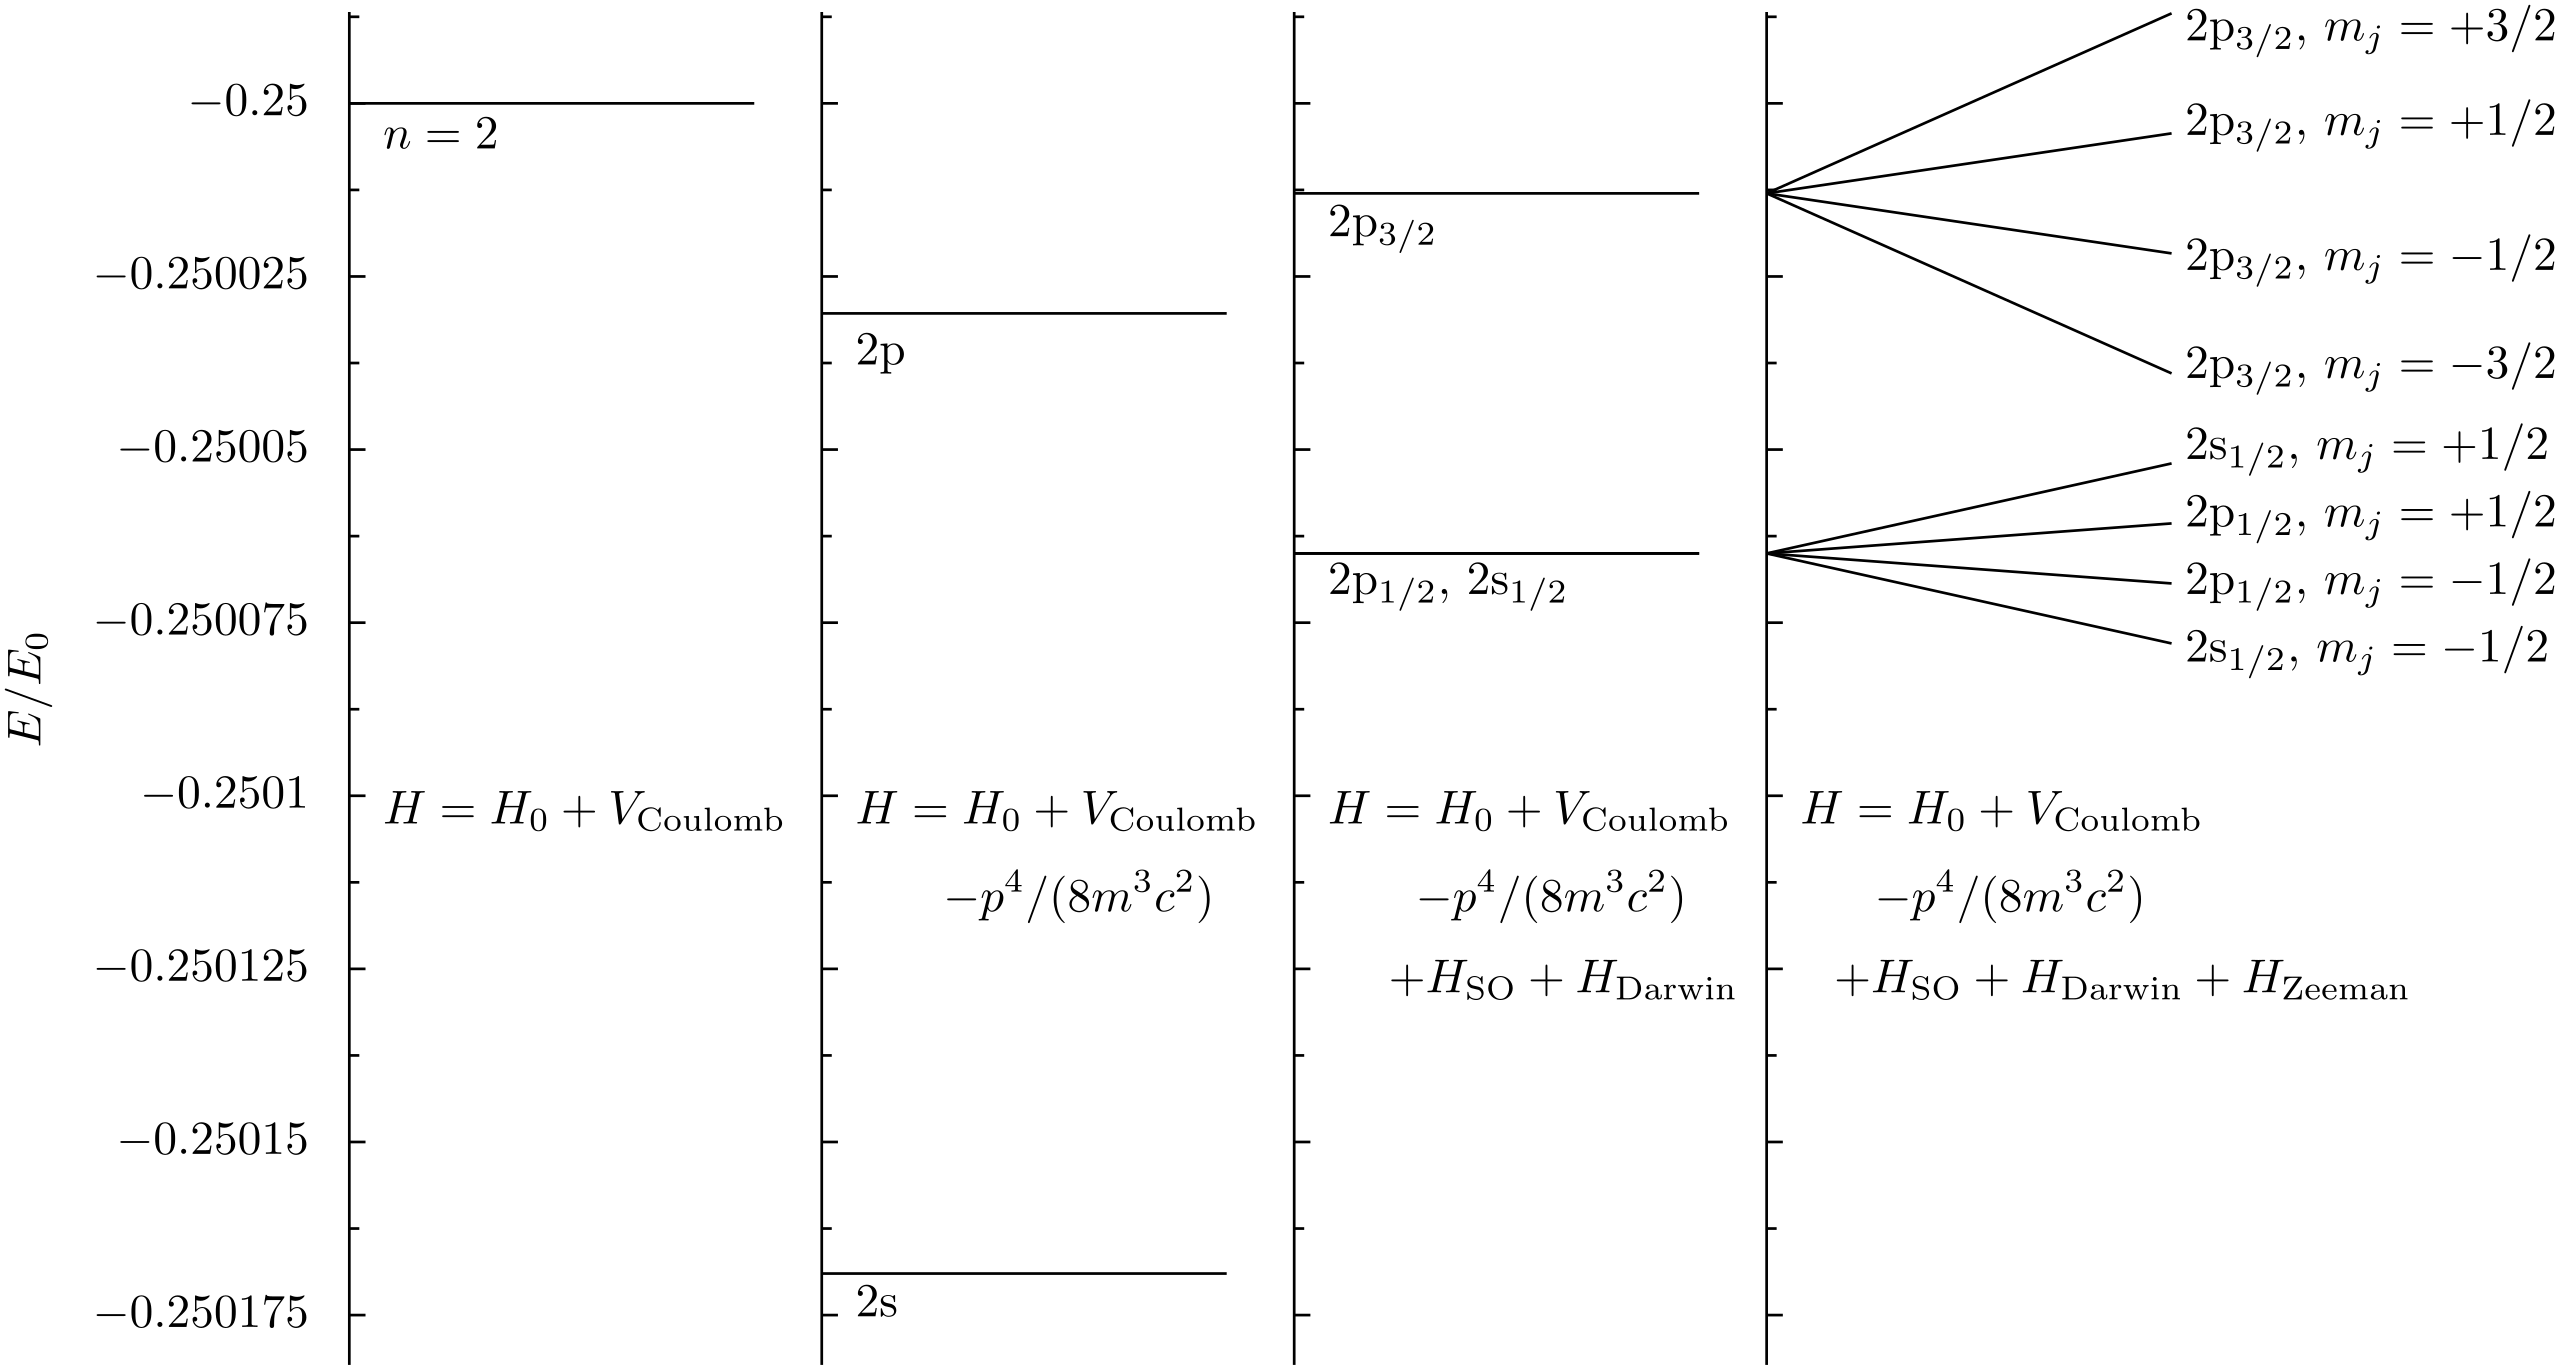
\includegraphics[width=\linewidth]{img/2560px-Hydrogen_fine_structure_energy_2.png}
    \caption{Visualisierung einiger Korrekturen der Feinstruktur bei Wasserstoff.
    Der Lamb-Shift ist hier noch nicht berücksichtigt.
    \refimgsource{Wikimedia}{https://commons.wikimedia.org/wiki/File:Hydrogen_fine_structure_energy_2.svg}{22.02.2022}{public domain}}
    \label{fig:feinstruktur wasserstoff}
\end{figure}

\begin{fquestion}{Woher weiß man, dass $2\mathrm{p}_{1/2}$ eine niedrigere Energie als $2\mathrm{p}_{3/2}$ hat?}
    Man kann ein externes Magnetfeld anlegen, um die Zustände unterscheiden zu können.
    Dabei spaltet sich $2\mathrm{p}_{3/2}$ in 4 Niveaus, und $2\mathrm{p}_{1/2}$ nur in 2 Niveaus auf.
\end{fquestion}

\begin{fquestion}{Strahlungskorrekturen veranschaulichen durch Zitterbewegung des Elektrons und Vakuumfluktuation?}
    (siehe Povh, Streuung und Strukturen, 4.1.3 und 4.2)
    
    \emph{Zitterbewegung}: Das Elektron ist nicht genauer als seine Compton-Wellenlänge $\Bar{\lambda}_e = \frac{\hbar}{m_ec}$ lokalisierbar.
    Das Potential wird dadurch verschmiert, was man über eine Unsicherheit $\delta\Vec{r}$ beschreiben kann.
    Da keine Richtung bevorzugt ist, folgt dann
    $$ V(\Vec{r} + \delta\Vec{r}) \equiv V(r) + \frac{1}{2} \frac{\nabla^2}{3}V(r) \langle (\delta\Vec{r})^2 \rangle  + \mathcal{O}(\delta\Vec{r}^4). $$
    Dabei gilt $\nabla^2 V(r) = 4\pi\alpha \delta (\Vec{r})$, die Korrektur ist also nur für S-Zustände relevant.
    Man erhält also das Störpotential $V_Z = \frac{2\pi \alpha}{3m_e^2} \delta (\Vec{r})$ (Im Erwartungswert gilt dann $\delta \rightarrow |\psi(0)|^2$).
    \\
    \emph{Lamb-Shift}: Es tragen zwei sogenannte Strahlungskorrekturen bei, Polarisation des Vakuums und Vakuumfluktuationen.
    Letztere liefert den Hauptbeitrag, man betrachtet den Einfluss der Fluktuation von $\Vec{E}$ auf $\delta \Vec{r}$.
    Genau wie bei der Zitterbewegung erhält man wieder über denselben Taylor-Ansatz eine Abschätzung der Korrektur.
    Allerdings ist die Herleitung der Vakuumfluktuation von $\Vec{E}$ etwas aufwendiger.
    Das Endergebnis im Povh ist 
    $$\Delta E_n = -E_n \frac{8\pi\alpha^3}{3n} \log \left( \frac{1}{\alpha^2} \right) > 0.$$
\end{fquestion}

\begin{fquestion}{Was passiert mit externem Magnetfeld, also Zeeman-Effekt?}
    Die Energieniveaus sind durch 
    $$\Delta E = -\Vec{\mu}\cdot\Vec{B}$$
    gegeben.
    Dabei kann man im schwachen Magnetfeld annehmen, dass $\Vec{L}$ und $\Vec{S}$ zum Gesamtdrehimpuls $\Vec{J}$ koppeln.
    Dann gilt
    $$\Vec{\mu} \simeq -\mu_Bg_J\frac{\Vec{J}}{\hbar}$$
    mit $\Vec{\mu}_J = g_L\Vec{\mu}_L + g_S\Vec{\mu}_S$ ($g_L = 1$ und $g_S \approx 2$).
    Der Lande-Faktor $g_J$ ist über
    $$\Vec{\mu}_J =: g_J\mu_B\Vec{J}$$
    definiert.
    Insbesondere ist also $g_J\Vec{J} = g_L\Vec{L} + g_S\Vec{S}$.
    Man kann zeigen, dass
    $$g_J = g_L \frac{J(J+1) + L(L+1) - S(S+1)}{2J(J+1)} + g_S \frac{J(J+1) - L(L+1) + S(S+1)}{2J(J+1)}.$$
    Betrachte dazu $\expval{\Vec{\mu}_J\cdot\Vec{J}} = g_J\mu_B\hbar^2 J(J+1)$ und andererseits
    $$g_J\expval{\Vec{J}\,^2} = \expval{g_L\Vec{L}\cdot\Vec{J} + g_S\Vec{S}\cdot\Vec{J}}, $$
    wobei $2\Vec{L}\cdot\Vec{J} = -(\Vec{J}-\Vec{L})^2 + \Vec{J}^2 + \Vec{L}^2 = \Vec{J}^2+\Vec{L}^2 - \Vec{S}^2$ (analog für den anderen Term).
    
    Qualitativ spaltet sich also $2p_{3/2}$ in $2J + 1 = 2\cdot \frac{3}{2} + 1 = 4$ Niveaus auf.
    Da $\Delta E = g_Jm_J\mu_B B$ haben Zustände mit höherem $m_J$ mehr Energie.
\end{fquestion}

\begin{fquestion}{Wann ist LS-Kopplung, wann jj-Kopplung relevant?}
    Grundsätzlich können wir den Hamiltonian als 
    $$H \equiv H_0 + \beta\frac{\expval{\Vec{L}\cdot\Vec{S} }}{r^3} + \gamma \Vec{J}\cdot\Vec{B}$$
    auffassen, wobei $\beta,\gamma$ hier irrelevante Vorfaktoren sind.
    Das Coulomb-Potential sei in $H_0$ enthalten, die anderen Terme modellieren dann jeweils die Spin-Bahn-Kopplung und die Wirkung eines externen Magnetfeldes.
    \\
    Ohne $\Vec{B}$-Feld und LS-Term wissen wir, dass die Eigenzustände durch $|nlm_lm_s\rangle$ beschrieben werden können.
    Unter Berücksichtigung der Spin-Bahn-Kopplung verwendet man stattdessen $|njm_j\rangle$.
    Solange der Zeeman-Term klein ist (also kleine $\Vec{B}$-Felder), können wir weiterhin $m_j$ als gute Quantenzahlen verwenden.
    Für große Felder ist der LS-Term dann vernachlässigbar, weshalb $m_l$ und $m_s$ wieder ``gute'' Quantenzahlen sind.
    Analog kann man durch den Vergleich von LS-Term und $H_0$ auch argumentieren, dass für leichte Atome LS-Kopplung vorliegt.
\end{fquestion}

\begin{fquestion}{Was passiert bei sehr hohen Magnetfeldern?}
    Entspricht dem Paschen-Back-Effekt, $L$ und $S$ koppeln nicht mehr.
    Die Energien sind jetzt $\Delta E = (g_lm_l + g_sm_s)\mu_B B$, da der Zeeman-Term den LS-Term dominiert.
\end{fquestion}

\begin{fquestion}{Was passiert bei dem Übergang von niedrigen zu hohen Feldern?}
    Für bestimmte Niveaus gibt es vermiedene Niveaukreuzungen (= AVL, avoided level crossing).
    Voraussetzung dafür ist, dass die Zustände ``dieselbe Symmetrie'' besitzen.
    Dann können sie mischen, und die Kreuzung vermeiden.
    Konkret bedeutet das, dass sich das $2\mathrm{p}_{3/2}$-Niveau mit $m_J = -\frac{3}{2}$ und das $2\mathrm{p}_{1/2}$-Niveau mit $m_J = \frac{1}{2}$ kreuzen, nicht aber das $2\mathrm{p}_{3/2}$-Niveau mit $m_J = -\frac{1}{2}$ und das $2\mathrm{p}_{1/2}$-Niveau mit $m_J = \frac{1}{2}$.
    Im letzteren Fall gilt $m_l = -1$ und $m_s = \frac{1}{2}$, bzw. $m_l = 1$ und $m_s = -\frac{1}{2}$ (siehe \autoref{fig:zeeman wasserstoff}).
    Für beide Kombinationen ist $m_l + 2m_s = 0$.
\end{fquestion}

\begin{figure}[!ht]
    \centering
    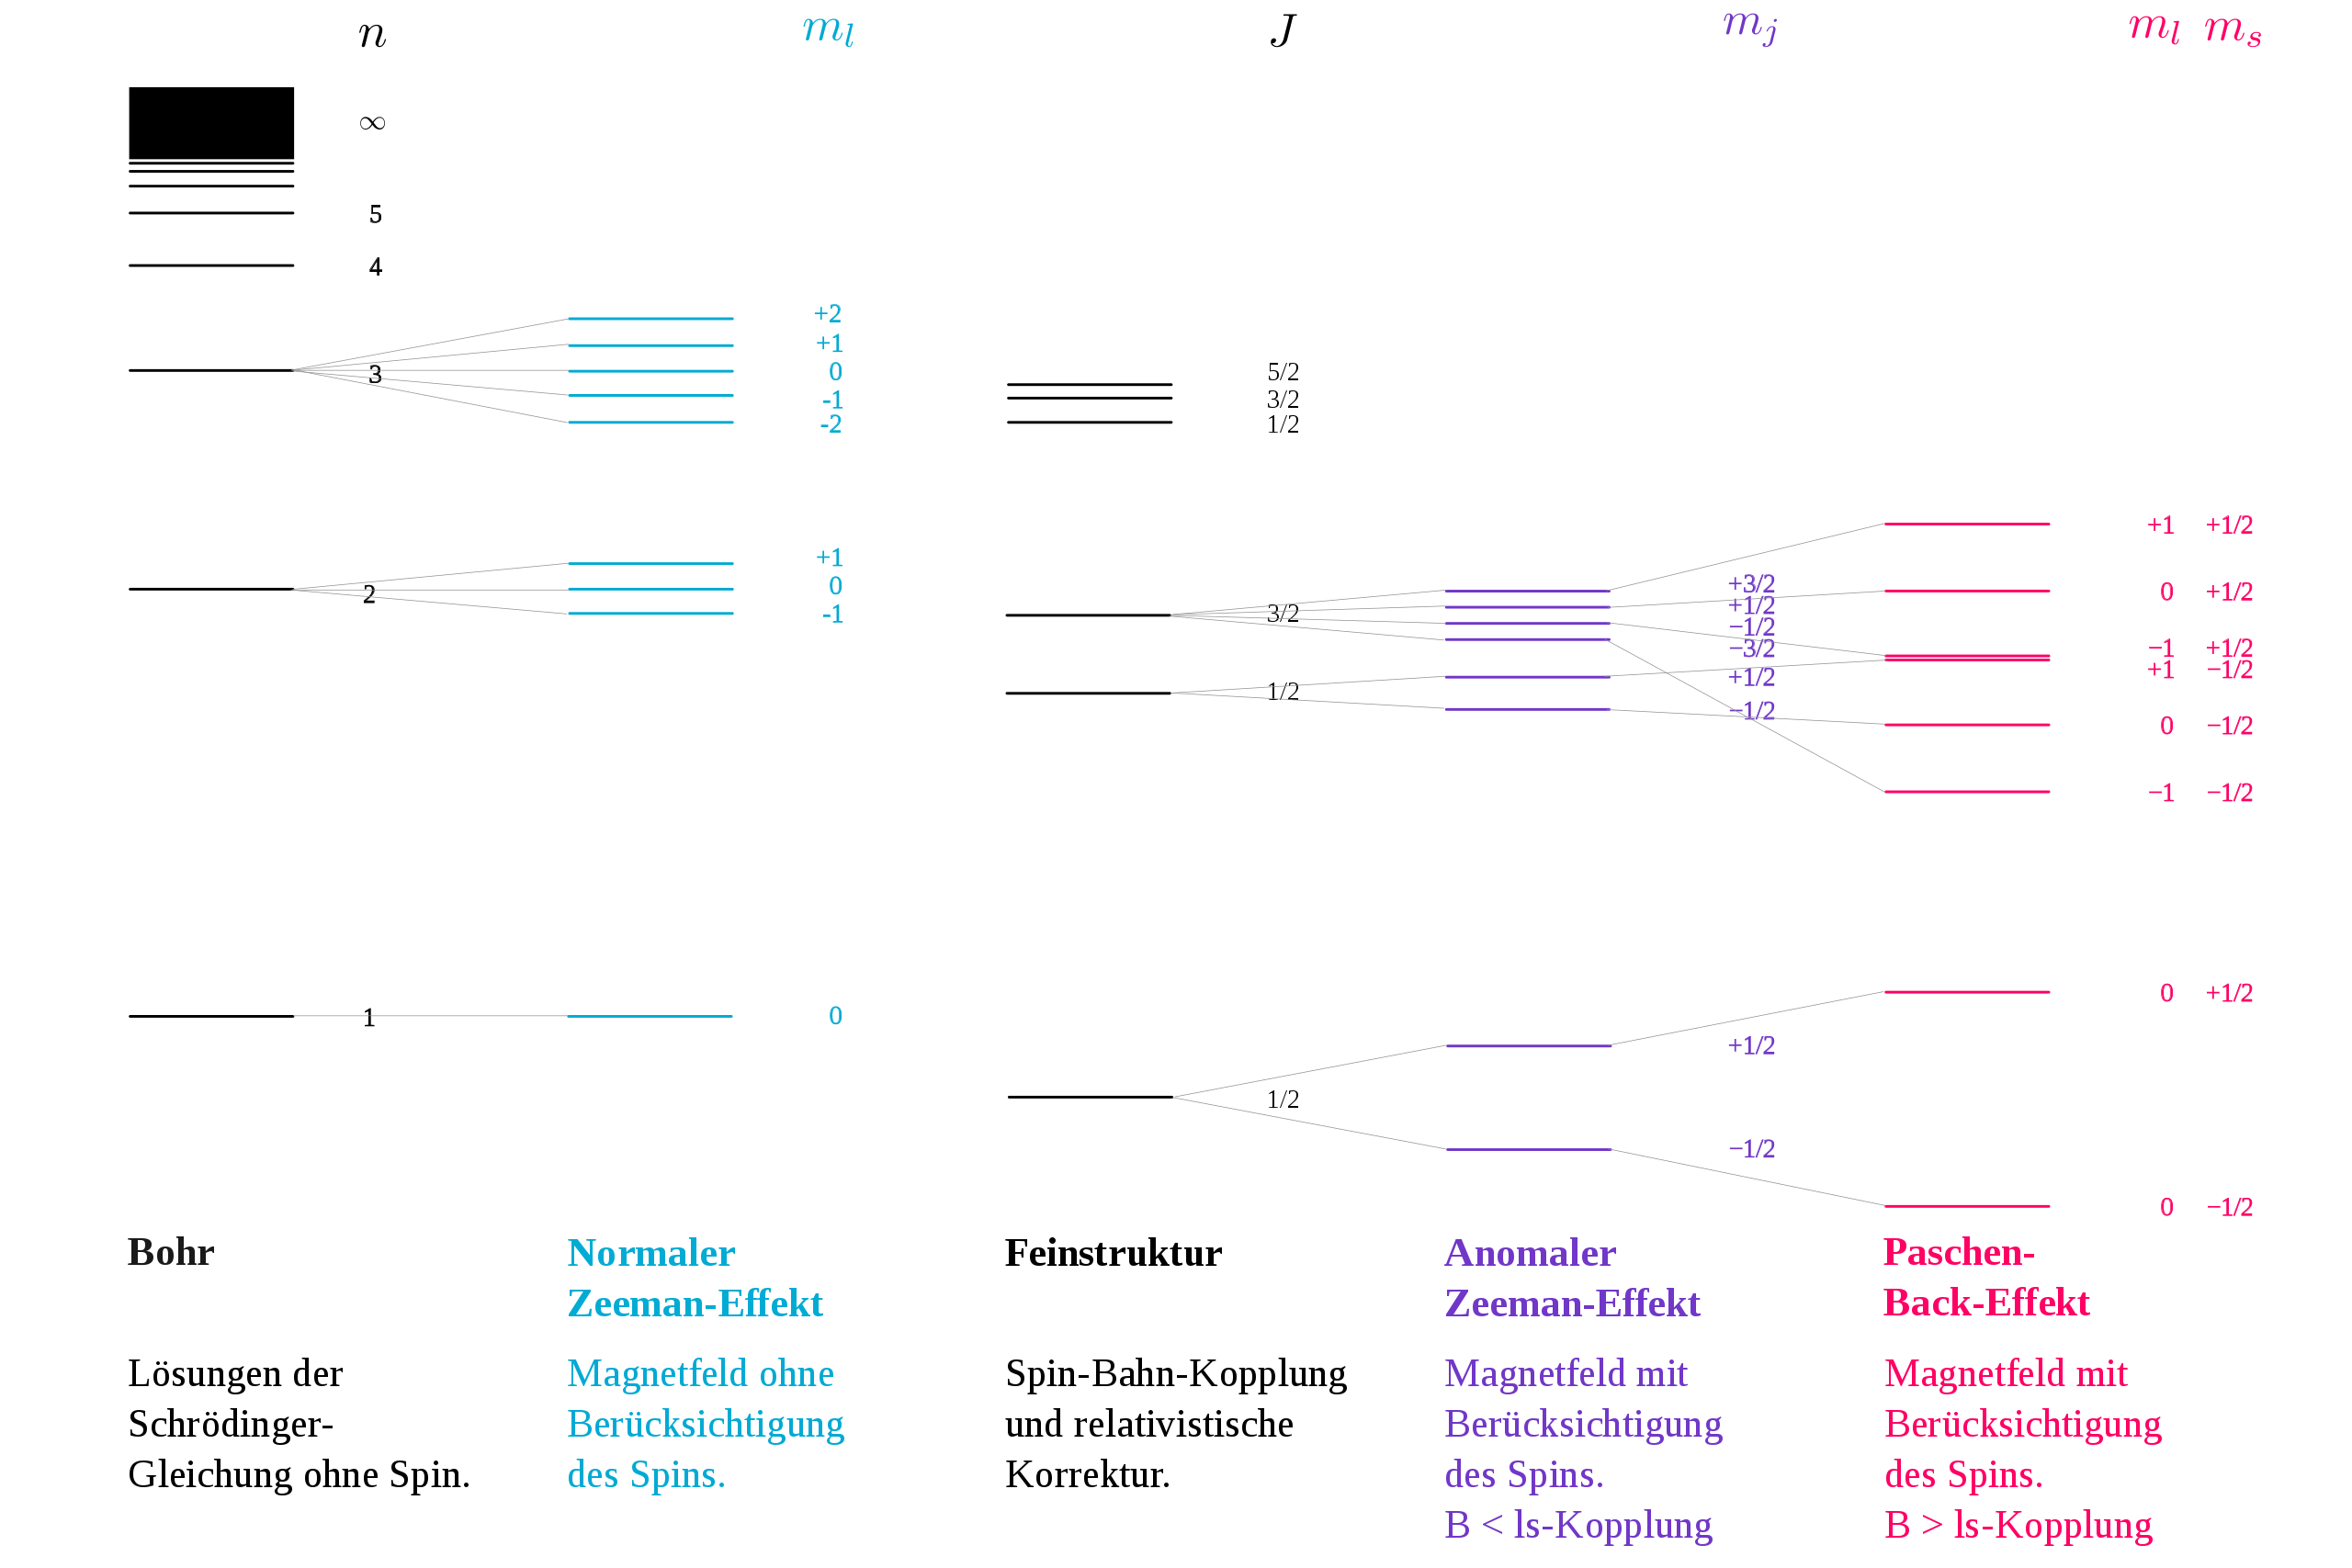
\includegraphics[width=\linewidth]{img/Wasserstoff_Zeeman.png}
    \caption{Aufspaltung der Energie-Niveaus von Wasserstoff in einem externen Magnetfeld (Zeeman-Effekt).
    \refimgsource{Wikimedia}{https://commons.wikimedia.org/wiki/File:Wasserstoff_Zeeman.svg}{22.02.2022}{public domain}}
    \label{fig:zeeman wasserstoff}
\end{figure}

% \begin{question}{Bei welchen Niveaus passiert das?}
%     $m_J = \pm\frac{3}{2}$ kreuzen sich, nur AVL für $m_J = \pm\frac{1}{2}$ ???
%     diese zwei Zustände vermeiden die Kreuzung, da für sie $m_l + 2m_s = 0$, sie wären also ohne Kopplung entartet ??? 
%     Kopplung fällt nur bei unendlichen Magnetfeldern weg, also Kreuzungspunkt im Unendlichen ???
% \end{question}

% \begin{question}{Wie kann man das mit AVL erklären?}
%     Die Zustände, die AVL machen, nähern sich so weit, dass sie nicht mehr zu unterscheiden sind
% \end{question}

\begin{fquestion}{Welche Größenordnung hat die Feinstruktur?}
    $E_{FS} \sim E_n \alpha^2 \sim \alpha^4$.
    $E_n$ in eV-Bereich, also $E_{FS}$ in meV-Bereich.
\end{fquestion}

\begin{fquestion}{Wie sieht das bei Atomkernen aus?}
    $E_n$ in MeV.
    Da $\alpha_s \sim 0.1-1$, liegt $E_{FS}$ auch im MeV-Bereich.
\end{fquestion}

\begin{fquestion}{Was hat das für Auswirkungen?}
    Dass die Feinstruktur in der gleichen Größenordnung wie die primäre Energieskala liegt hat eine starke Durchmischung der Energieniveaus zur Folge. 
    Um die magischen Zahlen vollständig zu erklären, muss die Feinstruktur berücksichtigt werden. 
    Zum Beispiel sorgt die Absenkung des $2f_{7/2}$ Niveaus für die magische Zahl 28. 
\end{fquestion}

% \begin{question}{Was gibt es denn noch für Quantenzahlen außer n?}
%     $l, s, m_l$ und $m_s$
% \end{question}

% \begin{question}{Warum sind $B$ und $L$ denn proportional, und wie?}
    
% \end{question}

\begin{fquestion}{Wie sieht das alles bei Mesonen aus, z.B. Charmonium?}
    Das Potential der starken Wechselwirkung kann hier als $V(r) = -\frac{4}{3} \frac{\alpha_s}{r} + kr$ angenommen werden, wobei $\alpha_s = \alpha_s(2m_\mathrm{charm}^\mathrm{const}) \approx 0.2$ mit der Konstituentenmasse $m_\mathrm{charm}^\mathrm{const} = \SI{1.5}{GeV}$.
    Für eine Abschätzung der Grundzustandsenergie kann man $k\simeq 0$ annehmen.
    Dann ist in Analogie zum Wasserstoff $E_0\approx \frac{\mu }{2}\left(\frac{4\alpha_s}{3} \right)^2 \approx \SI{27}{MeV} $, wobei $\mu = \frac{m_\mathrm{charm}^\mathrm{const}}{2}$ die reduzierte Masse ist (exp. Wert ist $\SI{32}{MeV}$, bei einer Gesamtmasse $\eta_\mathrm{charm}(1\mathrm{S} ) = \SI{2980}{MeV}$).
    
    In dieser Näherung wäre die maximale Masse $2m_\mathrm{charm}^\mathrm{const} = \SI{3}{GeV}$.
    Tatsächlich hat aber bereits der erste angeregte Zustand eine Masse von $\eta_\mathrm{charm}(2\mathrm{S} ) = \SI{3640}{MeV}$, was schematisch mit dem zusätzlichen linearen Term erklärt werden kann (Bindungszustände beliebig hoher Energie).
    
    % Grobstruktur erklären, Größenordnung $E_0$ mit $m_\text{charm}$ abschätzen ??? 
    % starke WW, also noch linearen Term im Potential für Confinement
\end{fquestion}

\begin{fquestion}{Woher kommt der Faktor $\frac{4}{3}$?}
    Es gibt drei Farbladungen und damit zunächst 9 mögliche effektive Gluonen
    $$|\mathrm{r}\overline{\mathrm{g}}\rangle, |\mathrm{r}\overline{\mathrm{b}}\rangle, |\mathrm{g}\overline{\mathrm{r}}\rangle, |\mathrm{g}\overline{\mathrm{b}}\rangle, |\mathrm{b}\overline{\mathrm{r}}\rangle, |\mathrm{b}\overline{\mathrm{g}}\rangle,
    |\mathrm{r}\overline{\mathrm{r}}\rangle,
    |\mathrm{g}\overline{\mathrm{g}}\rangle,
    |\mathrm{b}\overline{\mathrm{b}}\rangle.$$
    Da keine langreichweitige starke Wechselwirkung beobachtet wurde, kann es aber keines der farbneutralen Gluonen geben.
    Formal schließt man das ``weiße'' Gluon mit $\frac{1}{\sqrt{3}} (|\mathrm{r}\overline{\mathrm{r}}\rangle + |\mathrm{g}\overline{\mathrm{g}}\rangle + |\mathrm{b}\overline{\mathrm{b}}\rangle)$ aus.
    Üblicherweise werden die übrigen 8 Gluonen der SU(3) dann über 
    $$\begin{aligned} |\lambda_1\rangle &= \frac{1}{\sqrt{2}} (|\mathrm{r}\overline{\mathrm{b}}\rangle + |\mathrm{b}\overline{\mathrm{r}}\rangle ),&&&
    |\lambda_2\rangle &= \frac{-\i}{\sqrt{2}} (|\mathrm{r}\overline{\mathrm{b}}\rangle - |\mathrm{b}\overline{\mathrm{r}}\rangle ),\\
    |\lambda_3\rangle &= \frac{1}{\sqrt{2}} (|\mathrm{r}\overline{\mathrm{g}}\rangle + |\mathrm{g}\overline{\mathrm{r}}\rangle ),&&&
    |\lambda_4\rangle &= \frac{-\i}{\sqrt{2}} (|\mathrm{r}\overline{\mathrm{g}}\rangle - |\mathrm{g}\overline{\mathrm{r}}\rangle ),\\
    |\lambda_5\rangle &= \frac{1}{\sqrt{2}} (|\mathrm{b}\overline{\mathrm{g}}\rangle + |\mathrm{g}\overline{\mathrm{b}}\rangle ), &&&
    |\lambda_6\rangle &= \frac{-\i}{\sqrt{2}} (|\mathrm{b}\overline{\mathrm{g}}\rangle - |\mathrm{g}\overline{\mathrm{b}}\rangle ),\\
    |\lambda_7\rangle &= \frac{1}{\sqrt{2}} (|\mathrm{r}\overline{\mathrm{r}}\rangle - |\mathrm{b}\overline{\mathrm{b}}\rangle ),&&&
    |\lambda_8\rangle &= \frac{1}{\sqrt{6}} (|\mathrm{r}\overline{\mathrm{r}}\rangle +  |\mathrm{b}\overline{\mathrm{b}}\rangle - 2|\mathrm{g}\overline{\mathrm{g}}\rangle ) \end{aligned}$$
    dargestellt (siehe Gell-Mann-Matrizen $\lambda_{1\dots 8}$, die Indizierung ist manchmal anders). 
    Die ``hand-wavy'' Erklärung für den Faktor ist dann 
    $$\frac{1}{2} \Bigg[ \bigg\vert \underbrace{\frac{1}{\sqrt{2}}}_{|\lambda_1\rangle} \bigg\vert^2 + \bigg\vert \underbrace{\frac{-\i}{\sqrt{2}}}_{|\lambda_2\rangle} \bigg\vert^2 \Bigg] + \frac{1}{2} \Bigg[ \bigg\vert \underbrace{\frac{1}{\sqrt{2}}}_{|\lambda_3\rangle} \bigg\vert^2 + \bigg\vert \underbrace{\frac{-\i}{\sqrt{2}}}_{|\lambda_4\rangle} \bigg\vert^2 \Bigg] + \frac{1}{2} \Bigg[ \bigg\vert \underbrace{\frac{1}{\sqrt{2}}}_{|\lambda_7\rangle} \bigg\vert^2 + \bigg\vert \underbrace{\frac{1}{\sqrt{6}}}_{|\lambda_8\rangle} \bigg\vert^2 \Bigg] = \frac{4}{3}. $$
    Konzeptionell korrespondieren die Terme zu Feynman-Diagrammen, wo man üblicherweise die Betragsqudrate der Amplituden addiert. 
    % Die $\frac{1}{2}$-Faktoren sind jeweils von $\alpha_s$ abgespalten ??? 
    % Hier sind die Terme ausgehend von einem ursprünglich roten Quark aufgeschrieben.
    % ??? Wie sieht das in einem Feynman-Diagramm aus? 
    % Die Gluonen von oben existieren ja gar nicht, man zeichnet doch immer etwas wie rot-anti-blau ein etc. ??? 
    % ??? Wie kommt man damit jetzt auf die ``Rechnung'' aus der Vorlesung
\end{fquestion}

\begin{fquestion}{Was passiert bei kleinen Abständen?}
    Der lineare Term ist vernachlässigbar, man kann das Potential wieder (grob) als $\frac{1}{r}$-Potential ansehen und analog zum Coulomb-Potential vorgehen.
\end{fquestion}

\begin{fquestion}{Was passiert bei großen Abständen? }
    Der lineare Term führt zu einer beliebig großen Energie, bis genug für die Quark-Antiquark-Paarbildung vorhanden ist.
    Das erklärt dann phänomenologisch das Confinement, weil sich zwei Quarks nur so weit entfernen können, bis die Paarbildung auftritt.
    Es treten also nie ``isolierte'' Quarks auf.
\end{fquestion}

\begin{fquestion}{Welcher Effekt führt hier eigentlich zur Feinstruktur?}
    % starker Isospin ???  
    Die Aufspaltung der P-Zustände kann analog zum Wasserstoff-Atom über die Spin-Bahn-Kopplung erklärt werden.
    (siehe Povh 14.3, Quark-Antiquark-Potential)
\end{fquestion}

\begin{fquestion}{Was passiert bei der Hyperfeinstruktur?}
    Der Gesamtdrehimpuls $\Vec{J}$ koppelt an den Kernspin $\Vec{I}$ zum Gesamtspin $\Vec{F}$.
    Es dominieren zwei Effekte, die Kopplung des magnetischen Kernmomentes an das Magnetfeld des Elektrons, sowie das elektrische Quadrupolmoment des Kerns.
\end{fquestion}

\begin{fquestion}{Wie sieht die Kopplung des Kernmomentes aus?}
    Das Kernmoment ist $\Vec{\mu}_I = g_I\mu_N \Vec{I}$, mit dem Kernmagneton $\mu_N = \frac{e\hbar}{2m_p}$.
    
    Das Magnetfeld des Elektrons besteht aus einem Beitrag vom Bahndrehimpuls
    $$\Vec{B}_L = \frac{\mu_0}{4\pi r^3} 2\Vec{\mu}_L$$
    und einem Beitrag vom Spin durch $\Vec{A}_S = -\frac{\mu_0\Vec{\mu}_S}{4\pi} \times \nabla\frac{1}{r}$, also
    $$\Vec{B}_S = \nabla\times\Vec{A}_S = \frac{\mu_0}{4\pi r^3} \big[ 3(\Vec{\mu}_S\cdot \Vec{e}_r)\Vec{e}_r - \Vec{\mu}_S \big] + \frac{2\mu_0}{3}\Vec{\mu}_S\delta (\Vec{r}).$$
    (Der Faktor $\frac{2}{3}$ ergibt sich aus der Formel für das homogene Magnetfeld in einer Kugel oder einer rotierenden Kugel mit Oberflächenladung).
    
    Der distributionelle Anteil ist dabei nur für S-Zustände relevant, also für $L=0$.
    Die Energieänderung ist dann $\Delta E = -\Vec{\mu}_I \cdot (\Vec{B}_L + \Vec{B}_S)$.
\end{fquestion}

\begin{fquestion}{Gibt es die Hyperfeinstruktur auch nur für angeregte Zustände, wie bei der Feinstruktur und z.B. 2p?}
    Nein, gibt es auch bei $s_{1/2}$.
    Ein prominentes Beispiel ist die 21\,cm-Linie von Wasserstoff (entspricht 1420\,MHz).
    
    Allgemein gilt für Zustände mit $L=0$ näherungsweise eine vereinfachte Energiekorrektur.
    Diese ist
    $$\Delta E_\mathrm{HFS} \simeq \frac{2}{3} \expval{\Vec{\mu}_1\cdot\Vec{\mu}_2} |\psi (0)|^2 \equiv a \expval{\Vec{s}_1\cdot\Vec{s}_2},$$
    wobei $\Vec{\mu}_k = g_k \frac{g_\mathrm{int}}{2m_k} \Vec{s}_k$.
    Hierbei ist $g_\mathrm{int} = \sqrt{4\pi \alpha_\mathrm{int}}$ die Ladung der relevanten Wechselwirkung (für EM beispielsweise ist $g_\mathrm{int} \approx 0.3$).
    Mit $|\psi(0)|^2 = \frac{1}{\pi n^3r_0^3}$ und $r_0 = \frac{1}{m_\mathrm{red} \alpha_\mathrm{int}}$ findet man dann
    $$a = \frac{2}{3n^2} g_1g_2 \alpha_\mathrm{int}^4 \frac{m_\mathrm{red}^3}{m_1m_2}.$$
    
    Für das Elektron ist $g_s\approx 2$, für das Proton $g_s \approx 5.6$.
    In dieser Näherung findet ist $a \approx \SI{5.89}{\micro eV}$, was mit dem Umrechnungsfaktor $\frac{hc}{e} = \SI{1.24}{eV\,\micro m}$ einer Wellenlänge von
    $$\lambda = \frac{hc}{e}\cdot\frac{1}{a} \approx \SI{21}{cm}$$
    entspricht.
    % Eine höhere Genauigkeit kann man bei dieser Abschätzung nicht erwarten.
\end{fquestion}

\begin{fquestion}{Was ist denn mit dem Erwartungswert des Spin-Produktes passiert?}
    Für Wasserstoff ist $s_{1,2} = \frac{1}{2}$, also ist der Gesamtspin $S=1$ für parallele, und $S=0$ für anti-parallele Ausrichtung.
    Damit gilt 
    $$\langle \Vec{s}_1\cdot\Vec{s}_2\rangle = \frac{S(S+1) - s_1(s_1+1) - s_2(s_2+1)}{2} = \begin{cases} \frac{1}{4}, & \mathrm{parallel} \\ -\frac{3}{4}, & \text{anti-parallel} \end{cases}.$$
    Die Differenz zwischen den Energieniveaus erhält damit also gerade einen Faktor $\frac{1}{4} - \left(-\frac{3}{4}\right) = 1$, womit dann $\Delta E \equiv a$.
\end{fquestion}

\begin{fquestion}{Wie groß ist dann etwa das vom Elektron beim Proton induzierte Magnetfeld?}
    Es gilt $\Delta E \simeq \Vec{\mu}_p \cdot \Vec{B}_\mathrm{ind}$, die gesamte Aufspaltung ist also $a = 2\mu_p B_\mathrm{ind}$ (Differenz zwischen paralleler und anti-paralleler Ausrichtung).
    Damit ist dann 
    $$B_\mathrm{ind} = \frac{a}{2\mu_p} = \frac{a}{2\mu_B g_p} \frac{m_p}{m_e} \approx \SI{16.7}{T}.$$
\end{fquestion}

\begin{fquestion}{Wie beeinflusst ein schwaches externes Magnetfeld die Energieniveaus mit $S=0$ bzw. $S=1$?}
    Es gilt $\Delta E = -\Vec{\mu}_S\cdot\Vec{B}_\mathrm{ext}$, wobei gemäß Wigner-Eckart-Theorem
    $$\Vec{\mu}_S = \frac{\langle\Vec{\mu}_e\cdot\Vec{S} + \Vec{\mu}_p\cdot\Vec{S}\rangle}{\expval{\Vec{S}^2}} \Vec{S} \approx \frac{\langle\Vec{\mu}_e\cdot\Vec{S}\rangle}{S(S+1)} \Vec{S}.$$
    Dabei kann man das magnetische Moment des Protons vernachlässigen.
    Mit $\Vec{S} = \Vec{s}_e + \Vec{s}_p$ folgt daraus dann
    $$\Vec{\mu}_S = g_s\mu_B\Vec{S} \frac{s_e(s_e+1) + \langle\Vec{s}_e\cdot\Vec{s}_p\rangle }{S(S+1)} \approx \mu_B\Vec{S}, $$
    wobei $g_s\approx 2$.
    Damit ändern sich die Energieniveaus dann um $\Delta E \approx \mu_B B_\mathrm{ext} m_S$, mit $m_S=-1,0,1$.
    
    Anmerkung: Bei der Berechnung von $\Vec{\mu}_S$ muss man etwas aufpassen, ausführlich gilt
    $$\begin{aligned} \frac{2 \langle\Vec{s}_e\cdot\Vec{S}\rangle }{ \langle\Vec{S}^2\rangle } &= \frac{2s_e(s_e+1) +  S(S+1) - s_e(s_e+1) - s_p(s_p+1)}{S(S+1)} = \\
    &= \frac{S(S+1)}{S(S+1)}=1,\end{aligned}$$
    wobei auch für anti-parallele Spins $s_e=s_p=\frac{1}{2}$ ist, weshalb $s_e(s_e+1) - s_p(s_p+1) \equiv 0$!
\end{fquestion}

\begin{fquestion}{Wie beeinflusst ein starkes externes Magnetfeld die Energieniveaus mit $S=0$ bzw. $S=1$?}
    Hier koppeln $\Vec{\mu}_e$ und $\Vec{\mu}_p$ näherungsweise unabhängig voneinander an $\Vec{B}_\mathrm{ext}$, da $a$ gegenüber der Aufspaltung vernachlässigbar wird.
    Es gilt dann 
    $$\Delta E = (2\mu_B m_{s_e} - g_p \mu_N m_{s_p}) B_\mathrm{ext},$$ 
    wobei der zweite Term durch $\mu_N \ll \mu_B$ unterdrückt ist.
    Insbesondere ist das Vorzeichen umgekehrt wegen der Ladung des Protons umgekehrt.
\end{fquestion}

\begin{fquestion}{Warum ist die 21\,cm-Linie so interessant?}
    Das ist der Hyperfeinübergang des 1S Wasserstoffniveaus. 
    Bei diesem kommt es zu einem Spinflip, damit ist die Parität erhalten und kein elektrischer Dipolübergang ist möglich. 
    Ein magnetische Dipolübergang ist nötig. 
    Dieser ist unterdrückt. 
    Zudem ist die Photonenergie ca. $\SI{6}{\micro eV}$ und ist damit energetisch unterdrückt. 
    Dieser Zustand hat durch diese Unterdrückung eine Lebensdauer von ca. $11$ Millionen Jahren und eine sehr scharfe Spektrallinie (Lange Lebensdauer $\rightarrow$ scharfer Peak). 
    Daher kann diese Linie zur Vermessung von Geschwindigkeiten von Wasserstoffansammlungen im Universum über den Dopplereffekt benutzt werden. 
\end{fquestion}

\begin{fquestion}{Warum mögen Astrophysiker keine Handys?}
    Handyfrequenzen liegen im Bereich $(0.8 -3.6)\,$GHz und somit im gleichen Frequenzbereich wie der Wasserstoff-Hyperfeinübergang mit $1.420\,$GHz. 
\end{fquestion}

\begin{fquestion}{Woher weiß man bei den Radioteleskopen auf der Erde, dass der Wasserstoff nicht aus der Atmosphäre kommt?}
    Die strahlungslose Abregung durch Stöße ist viel schneller, da Stöße bei irdischen Dichten viel häufiger stattfinden. 
    Daher findet der Hyperfeinübergang hier nicht statt. 
\end{fquestion}

\subsection{Atomkern}

\begin{fquestion}{Was sind die typischen Kernenergien?}
    Typische Bindungsenergien pro Nukleon sind $(7-8)$\,MeV.
    Die Potentialtiefe wächst kontinuierlich von 17\,MeV (Lithium) bis 44\,MeV (Blei) mit der Massenzahl $A$ an.
    Der Fermi-Impuls beträgt etwa 250\,MeV (siehe Povh 6.3).
    Die Energieniveaus wachsen etwa quadratisch (Kastenpotential, also $E_n\sim n^2$).
    Die Fermi-Energien betragen etwa $E_F \approx \frac{p_F^2}{2M} \approx 33$\,MeV (siehe Povh 18.1).
\end{fquestion}

\begin{fquestion}{Wie bestimmt man die Fermi-Energie?}
    Quasieleastische Streuung an Wasser. 
    Über den Abstand des Peaks der im Sauerstoff gebundenen Protonen mit den ``freien'' Protonen kann man die Bindungsenergie bestimmen. 
    Über die Breite des Peaks der gebundenen Protonen kann man den Fermi-Impuls bestimmen, da die Verbreiterung des Peaks durch die Bewegung der Protonen im Kern kommt, diese haben dabei den Fermi-Impuls. 
\end{fquestion}

\begin{fquestion}{Was hat es mit dem Tröpfchenmodell auf sich?}
    Die Bethe-Weizsäcker-Formel lautet
    $$E_B = a_V A - a_O A^{2/3} - a_C \frac{Z^2}{A^{1/3}} - a_A \frac{(N - Z)^2}{A} + \delta(N, Z)$$
    Man betrachtet fünf Beiträge zur Bindungsenergie
    \begin{enumerate}
        \item \emph{Volumenenergie}: $a_VA$, proportional zur Anzahl der Nukleonen $A$.
        Durch die kurze Reichweite der starken Wechselwirkung gibt es keinen $A^2$-Term, den man beispielsweise für die Coulomb-Wechselwirkung erwarten würde.
        Effektiv trägt nur die Wechselwirkung mit nächsten Nachbarn bei.
        \item \emph{Oberflächenenergie}: $-a_OA^{2/3}$, proportional zur Oberfläche des Kerns (also $\propto R^2$).
        Nukleonen an der Oberfläche haben weniger nächste Nachbarn, was zu einer geringeren Bindungsenergie führt.
        \item \emph{Coulombterm}: $-a_C \frac{Z^2}{A^{1/3}}$, proportional zum Quadrat der Anzahl an Protonen.
        Der Faktor $A^{-1/3}$ entspricht der $\frac{1}{R}$-Abhängigkeit.
        \item \emph{Asymmetrieterm}: $-a_A \frac{(N-Z)^2}{A}$ proportional zum Quadrat der Differenz von Neutronen und Protonen. 
        Qualitativ beruht er auf dem Pauli-Prinzip.
        Falls ein Kern deutlich mehr Protonen als Neutronen besitzt, könnte die Energie durch Umwandlung der höher liegenden Neutronen in Protonen verringert werden.
        \item \emph{Paarungsterm}: $\frac{\delta}{A^{1/2}} $ für gg-Kerne, $-\frac{\delta}{A^{1/2}} $ für uu-Kerne und 0 für gu-Kerne (g: gerade, u: ungerade).
    \end{enumerate}
    Die Parameter eines least-squares fit sind etwa $a_V \approx 16\,$MeV, $a_O \approx 18\,$MeV, $a_C \approx 0.7\,$MeV, $a_A \approx 23\,$MeV und $\delta \approx 12\,$MeV.
    Siehe \autoref{fig:experimental-mass-binding-model} für einen Plot der Bindungsenergie pro Nukleon.
\end{fquestion}

\begin{figure}[!ht]
    \centering
    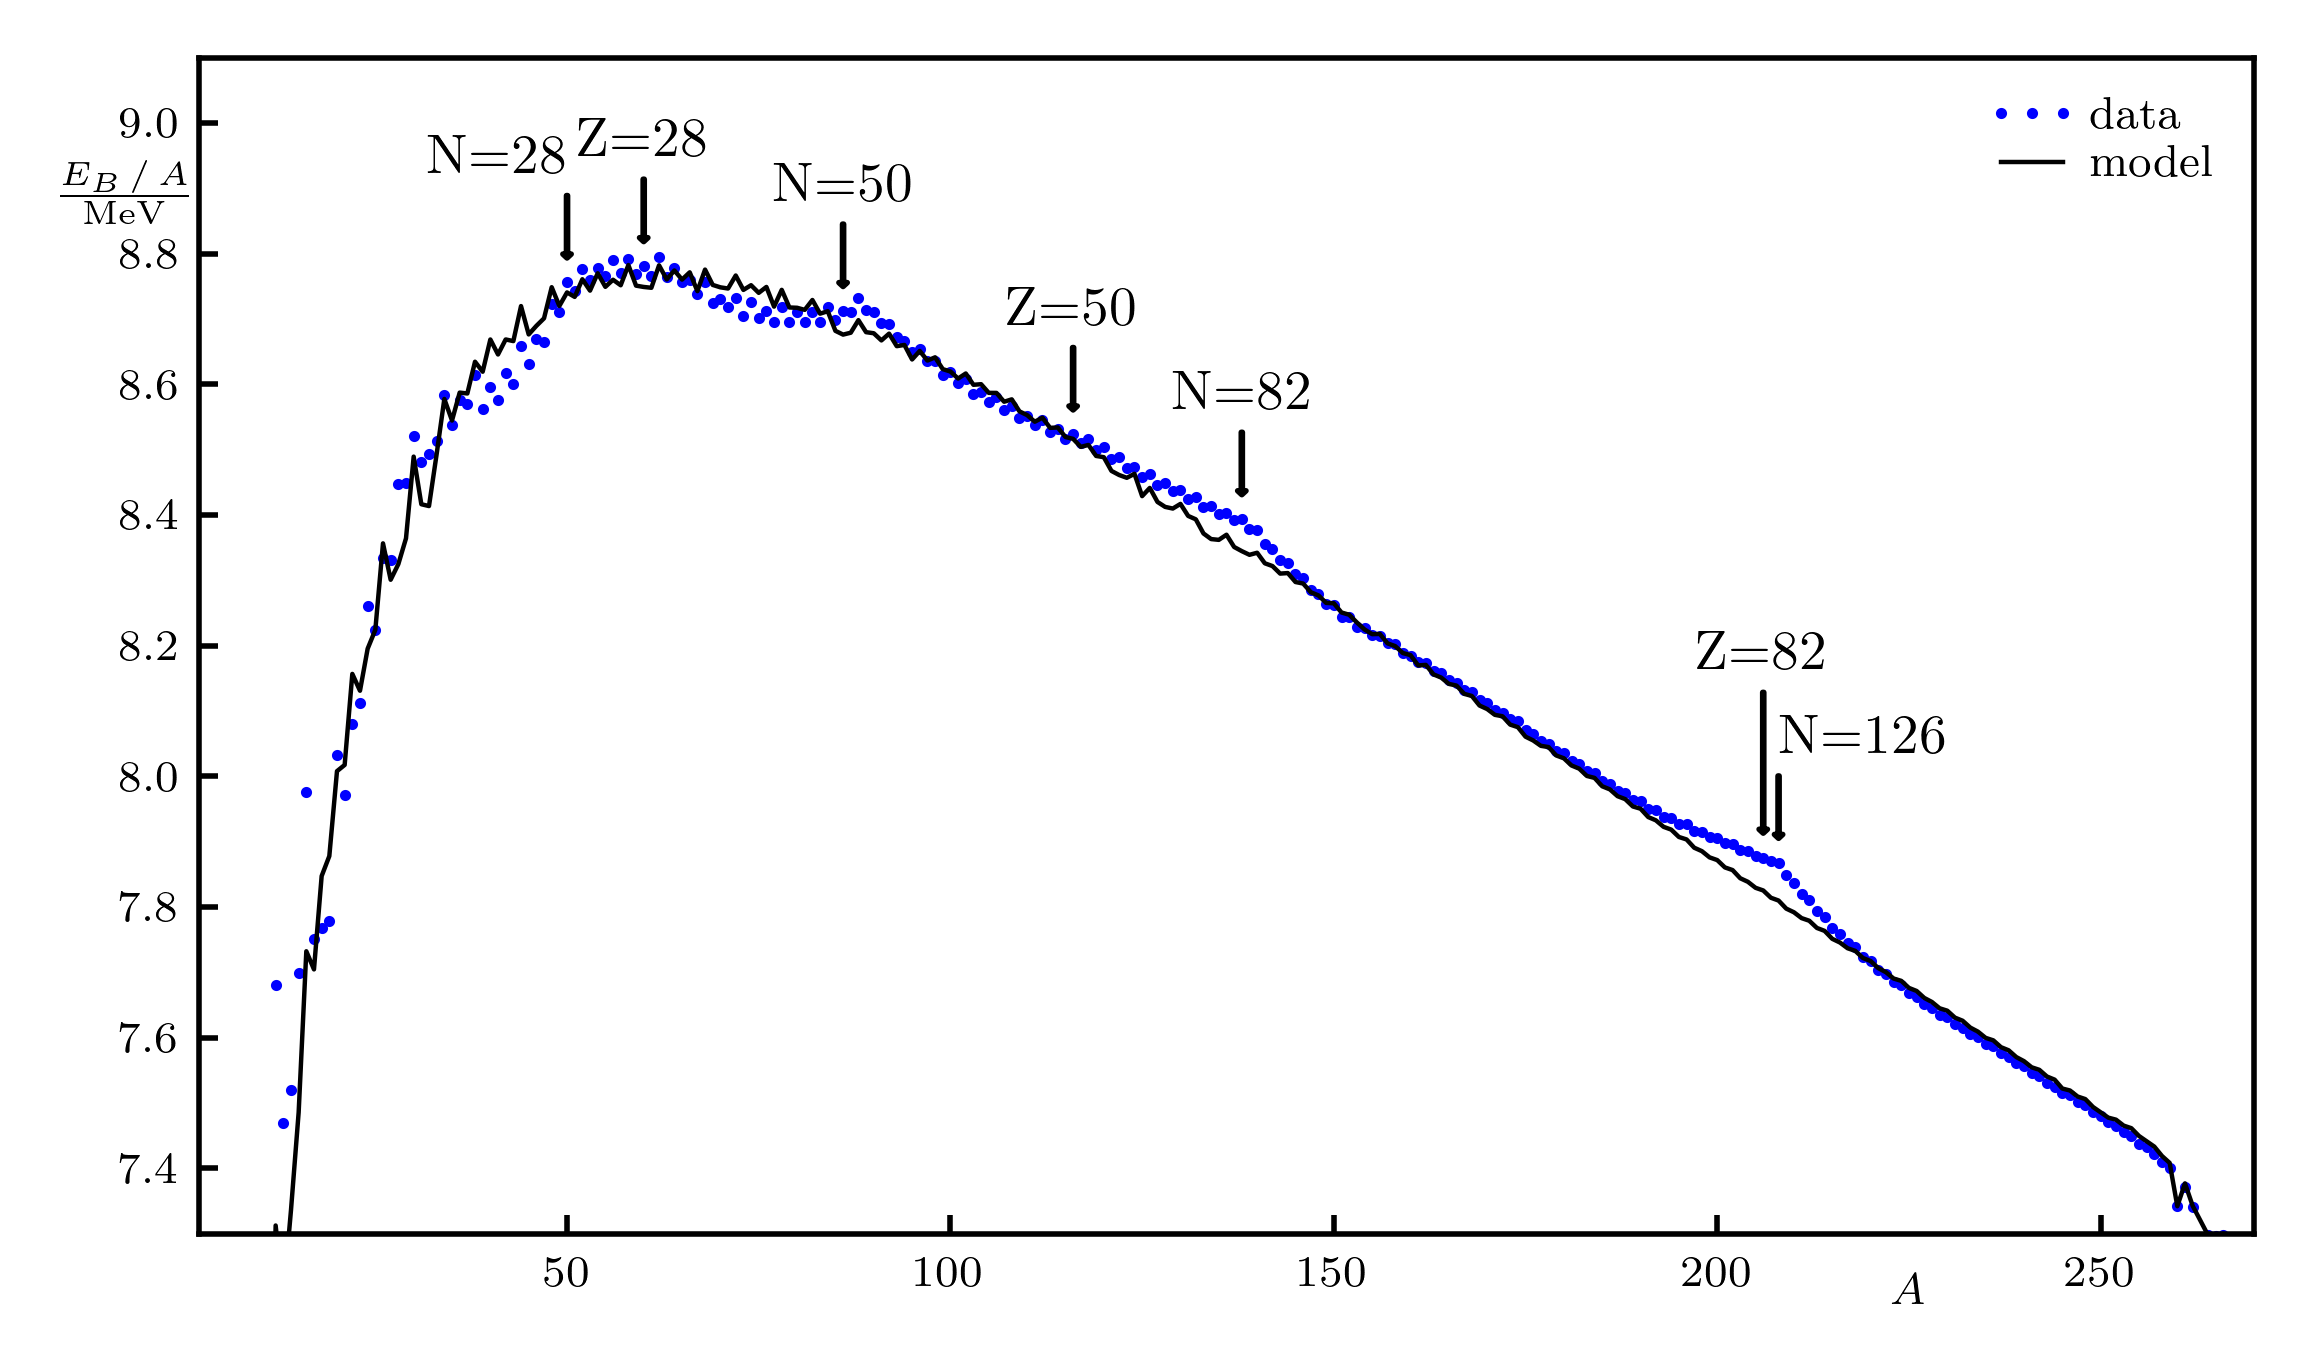
\includegraphics{img/experimental-mass-binding-model2.png}
    \caption{Plot der semi-empirischen Massenformel für $a_V = 15.75\,$MeV, $a_O = -17.8\,$MeV, $a_C = -0.711\,$MeV, $a_A = -23.7\,$MeV und $\delta = 11.18\,$MeV.
    Die experimentellen Daten sind aus \cite{WanAudKonHuaNaiXu2016} entnommen und entsprechen jeweils der maximalen Bindungsenergie pro Nukleon für die jeweilige Massenzahl $A$. }
    \label{fig:experimental-mass-binding-model}
\end{figure}

\begin{fquestion}{Was hat es mit den Zacken im $E_B / A$-Bild auf sich?}
    Die Zacken entsprechen den sogenannten magischen Zahlen (2, 8, 20, 28, 50, 82, 126).
    Dabei gibt es eine erhöhte Bindungsenergie, die mit dem Schalenmodell des Kerns erklärt werden kann.
\end{fquestion}

\begin{fquestion}{Wie kommt man darauf?}
    Die ersten drei Zahlen kann man als abgeschlossene Schalen interpretieren.
    Analog zum Atommodell gibt es $2(2\ell +1)=2,6,10,\dots$ Zustände, damit entsprechen $2,8,20$ den Schalen $1\mathrm{s},1\mathrm{p},2\mathrm{s}$.
    Für die höheren magischen Zahlen muss dann die Spin-Bahn-Wechselwirkung beachtet werden.
    % Durch die (numerische) Lösung der Schrödingergleichung.
\end{fquestion}

\begin{fquestion}{Wieso kann man nicht einfach mit dem Tröpfchenmodell den Kern beschreiben? }
    Die Spin-Bahn-Wechselwirkung ist so stark, dass sie die Energieniveaus im Schalenmodell stark beeinflusst.
    Beispielsweise kann die magische Zahl 28 erst durch die enorme Aufspaltung des 1f-Orbitals erklärt werden.
    Dabei liegt $1f_{7/2}$ so viel tiefer, dass es eine große Energielücke zum nächsten Orbital gibt. 
    Da $1f_{7/2}$ mit acht Nukleonen besetzt werden kann, erhält man ausgehend von der magischen Zahl 20 dann die 28 (siehe Povh Abb. 18.7).
\end{fquestion}

\begin{fquestion}{Wie ist die Spin-Bahn-Wechselwirkung bei Elektronen und bei Nukleonen?}
    Es ist $V(r) = V_\text{Woods-Saxon} + V_{l s}\langle \Vec{l} \cdot\Vec{s}\rangle $.
    Dabei erhält man eine Energieaufspaltung von $\Delta E_{ls} = \frac{2l+1}{2} \langle V_{ls} \rangle$.
    Im Gegensatz zum Atom ist hier $\langle V_{ls} \rangle < 0$ (anziehend), also liegen die Zustände mit $j = l + \frac{1}{2}$ immer unter denen mit $j = l - \frac{1}{2}$.
\end{fquestion}

\begin{fquestion}{Wie sieht das Potential eines Kerns aus?}
    Für größere Kerne ist das Woods-Saxon-Potential eine gute Näherung, wobei
    $$V(r) = \frac{-V_0}{1 + \e^{(r-r_0) / a}}$$
    mit der Potentialtiefe $V_0 \approx (40-50)\,$MeV, dem mittleren Radius $r_0 \approx 1.2\,\mathrm{fm}\cdot A^{1/3}$ und dem Parameter $a\approx 0.5\,$fm (beschreibt die Ausdehnung des Randes). 
    
    
    Das Woods-Saxon-Potential für einen Kern mit $A \approx 50$ ($r_0 = \SI{4.6}{fm}$ und $a = \SI{0.5}{fm}$.
    \begin{center}
        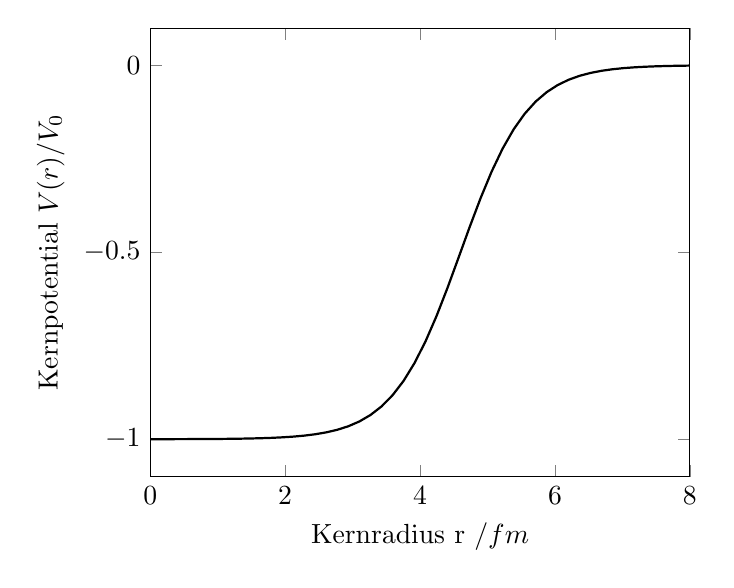
\begin{tikzpicture}
            \begin{axis}[domain=0:8, xmin=0, xmax=8, ytick distance = 0.5, xlabel={Kernradius r $/ \si{fm}$}, ylabel={Kernpotential $V(r) / V_0$}]
                \addplot [thick, black, samples=50] {-1 / (1 + exp((x-4.6)/0.5)};
            \end{axis}
        \end{tikzpicture}
    \end{center}
\end{fquestion}

% \begin{question}{Wieso gibt es im Woods-Saxon keinen Abstoßungsterm?}
%     weil es ein gemitteltes Potential ist ??? 
%     die Reichweite der Pion-WW reicht nur für nächste Nachbarn
%     Oberflächeneffekte wichtig, da weniger nächste Nachbarn (führt zu diffusem Rand ??? )
% \end{question}

\begin{fquestion}{Wie sieht das Woods-Saxon-Potential für kleinere und größere Kerne aus?}
    Kleine Kerne sind eher gaussförmig, hier ist Woods-Saxon keine gute Näherung. 
    Für größere Kerne wird das Woods-Saxon-Potential breiter, aber nicht tiefer. 
\end{fquestion}

\begin{fquestion}{Wieso wird es nicht tiefer?}
    Bei der Nukleonenbindung tragen nur die nächsten Nachbarn zur Wechselwirkung bei, weil die Nukleon-Nukleon-Bindung über Pionen eine kurze Reichweite hat.
\end{fquestion}

\begin{fquestion}{Wie sieht das Potential für ein Elektron in einem großen Atom aus?}
    Für größere Atome (bspw. prominent die Alkalimetalle) definiert man zunächst eine effektive Kernladungszahl $Z_{\mathrm{eff}}(r)$ durch die das Coulomb-Potential die Form
    $$V(r) = \frac{1}{4\pi\epsilon_0} \frac{Z_{\mathrm{eff}}(r) e^2}{r}$$
    annimmt.
    Da die Abschirmung der Kernladung durch die anderen Elektronen vom Abstand zum Kern abhängt, erwartet man folgende Grenzwerte:
    $$Z_{\mathrm{eff}} \xrightarrow{r \rightarrow 0} Z \quad\text{und} \quad Z_{\mathrm{eff}} \xrightarrow{r \rightarrow \infty} 1.$$
    Beispielweise kann die effektive Kernladung durch den folgenden ``reasonable guess'' für Natrium von C.J. Foot aus Atomic Physics oder das Yukawa-Potential modelliert werden.
    \begin{center}
        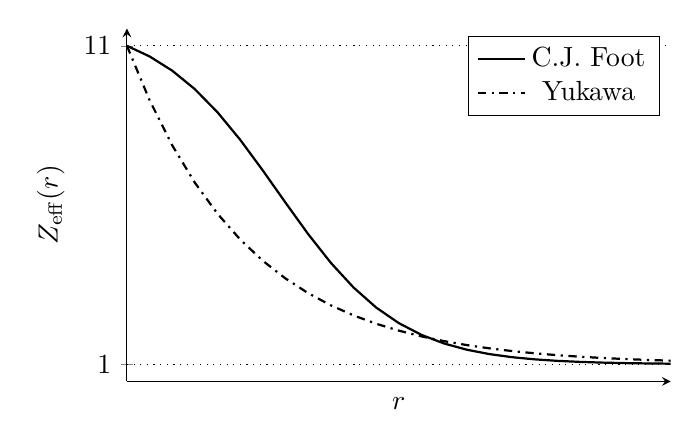
\begin{tikzpicture}
        [
            declare function = {
                f(\x) = 1+10/(1+exp(0.2*\x-2.5));
                yukawa(\x) = 1 + (f(0) - 1) * exp(-0.1 * \x);
            }
        ]
            \begin{axis}[xmin=0, xmax=45, ytick={1, f(0)}, ymin=0.5, ymax={f(0)+0.5}, yticklabels={$1$, $11$}, xtick=\empty,  xlabel={$r$}, ylabel={$Z_{\mathrm{eff}}(r)$},axis y line = left, axis x line = bottom, x axis line style = {-stealth}, y axis line style = {-stealth}, width=0.7\linewidth,height=0.5\linewidth]
                \addplot[domain=0:45, thick]{f(x)};
                \addlegendentry{C.J. Foot}
                \addplot[domain=0:45, thick, dash dot]{yukawa(x)};
                \addlegendentry{Yukawa}
                
                \addplot[domain=0:45, dotted]{f(0)};
                \addplot[domain=0:45, dotted]{1};
            \end{axis}
        \end{tikzpicture}
    \end{center}
\end{fquestion}

\begin{fquestion}{Sieht das Potential für Protonen und Neutronen unterschiedlich aus?}
    Ja, weil sich die Protonen noch über die Coulomb-Wechselwirkung abstoßen. 
    Das Potential der Neutronen ist also etwas tiefer.
    
    Dies spielt beim $\alpha$-Zerfall eine Rolle, weil diese eine Ladung $2+$ haben.
\end{fquestion}

% \begin{question}{Bei welchem Zerfall spielt das eine Rolle?}
%     alpha-Zerfall, Heliumkerne haben Ladung 2+
% \end{question}

\begin{fquestion}{Wieso fliegen überhaupt Heliumkerne raus?}
    Kern ist doppelt magisch, hat also eine sehr hohe Bindungsenergie.
    Dadurch wird die Tunnelbarriere verringert, was den $\alpha$-Zerfall in den meisten Fällen am wahrscheinlichsten.
    
    Relevant bei der spontanen Spaltung sind die Änderung von Coulomb- und Oberflächen-Energie
    $$\Delta E = a_C \frac{Z^2}{A^{1/3}} + a_O A^{2/3} \overset{!}{<} 0.$$
    Umformen liefert $\frac{A}{Z^2} > \frac{a_C}{-a_O} \approx 0.04$.
    Bei genauerer Abschätzung erhält man noch einen Faktor 2, also $\frac{Z^2}{A} > \frac{-2a_O}{a_C} \approx 48$.
    Das ist erfüllt für $Z>114$ und $A> 270$ (siehe Povh, 3.3 Kernspaltung).
\end{fquestion}

\begin{fquestion}{Wie sieht das Deuteron-Potential aus?}
    Das Deuteron ist der gebundene Zustand von Neutron und Proton.
    Seine Bindungseigenschaften werden im Povh durch ein Kastenpotential beschrieben.
\end{fquestion}

% \begin{question}{Wie sieht das Potential des Deuterons aus (bzw. allgemein für nur 2 Nukleonen im Kern)?}
%     Yukawa mit Abstoßungsterm für Spin-Spin-WW (** Im Povh steht zum Deuteron, dass auf die Quarks nicht das Pauli-Prinzip wirkt, weil die Farbladungen immer noch für unterschiedliche Zustände sorgen können. Stattdessen soll durch die starke Spin-Spin-WW ein ähnlicher Effekt wie Pauli entstehen ??? )
% \end{question}

\begin{fquestion}{Wie sind die Größenordnungen des Deuteron-Potentials?}
    Im Grundzustand des Deuterons gilt
    {
    \begin{align*}
        & \text{Topfvolumen} & Va^2 &\approx \SI{100}{MeV fm^2} \\
        & \text{Effekt. Ausdehnung} & a &\approx \SIrange{1.2}{1.4}{fm} \\
        & \text{Potentialtiefe} & V &= \SI{50}{MeV} \\
         &\text{Bindungsenergie} &  B &=\SI{2.225}{MeV} \\
        &\text{Spin und Parität} & J^P &= 1^+ \\
        &\text{Isospin} & I &= 0 \\
        &\text{Magnetisches Moment} & \mu &= 0.857 \mu_N \\
        &\text{Elektr. Quadrupolmoment} & Q&=\SI{0.282}{e fm^2}
    \end{align*}
    }
    Die Werte sind aus unerändert aus dem Povh entnommen.
\end{fquestion}

\begin{fquestion}{Welche Kräfte charakterisieren die Kernkraft?}
    Der abstoßende Teil wird entweder durch ein Pauliverbot oder Spinwechselwirkungen der Konstituentenquarks erklärt.
    
    Der anziehende Teil wird entweder ähnlich zur kovalenten Bindung bei Molekülen durch den Austausch eines zweier gleichfarbiger Quarks zwischen zwei Nukleonen oder einen Quark-Antiquark-Austasuch (in Form des Yukawa-Terms) begründet.
\end{fquestion}

\begin{fquestion}{Wie sieht der Yukawa-Teil aus?}
    Der Yukawa-Teil charakterisiert das Potential des Mesonen-Austauschs.
    Er hat die Form
    \[V(r) = g \frac{e^{-mcr}}{r}\]
    mit der Pionenmasse $m = \SI{139}{MeV}$.
    Er ergibt sich als Lösung der Klein-Gordon-Gleichung für ein Teilchen der Masse $m$ im statischen Potential.
\end{fquestion}

\begin{fquestion}{Wieso gibt es denn eine Pauli-Abstoßung von Neutron und Proton?}
    Allgemein besitzen beide eine Unterstruktur aus Quarks, die als Fermionen dem Pauliverbot unterliegen. 
    Dabei kann jedes der Quarks zwei Spin ($\uparrow, \downarrow$) Zustände, zwei Isospinzustände ($u$-Quark, $d$-Quark) und drei Farbzustände ($r, g, b$) einnehmen.
    Somit ist der gleiche Energiezustand $2 \cdot 2 \cdot 3 = 12$-fach entartet. 
    
    Sind nur zwei Nukleonen mit jeweils drei Quarks beteiligt, folgt daraus entsprechend keine Abstoßung.
    Hier folgt die Abstoßung aus der Ausrichtung der Spins
\end{fquestion}

\begin{fquestion}{Warum gibt es eigentlich keine Diprotonen?}
    Die starke Wechselwirkung ist abhängig vom Spin, und insbesondere anziehend für parallele Ausrichtung.
    Für zwei Protonen oder Neutronen muss der Spin aufgrund des Pauli-Prinzips aber entgegengesetzt sein, daher gibt es keine entsprechenden Bindungszustände.
    Bei Deuterium gibt es dieses Problem nicht.
\end{fquestion}

% \begin{question}{Was ist abgesehen von der Bindungsenergie an doppelt magischen kernen besonders?}
%     sind kugelsymmetrisch, also keine Rotationsanregungen (hand-wavy: Anregung in QM mit Ableitung verknüpft, Rotation also nur bei $\phi$-Abhängigkeit)
% \end{question}

% \begin{question}{Sind das nicht alle Kerne?}
%     nein, die sind durch die Valenznukleonen deformiert, über Rotationsanregungen messbar
% \end{question}

% \begin{question}{Was kann man messen, wenn man ein Neutron mit einigen MeV hat?}
%     Formfaktor von Kernen ??? 
% \end{question}

% \begin{question}{Wie kann man die Niveaus messen?}
%     Spektroskopie mit Photonen, siehe Photoeffekt
% \end{question}

\subsection{Wasserstoffmolekülion}

\begin{fquestion}{Welche Anregungen gibt es für Moleküle?}
    Bei einem Molekül kann eine Anregung des inneren Zustands, also eine Erhöhung der Energie bei ruhendem Massenmittelpunkt, auf drei Arten stattfinden:
    \begin{enumerate}
        \item elektronische Anregung $\sim E_0 = \frac{m_e}{2}\alpha^2 \lesssim \SI{10}{eV}$ (durch verschiedene Anregungszustände der Elektronen im Molekül),
        \item Vibrations-Anregung $\sim E_0\sqrt{\frac{m_e}{m_\mathrm{red}}} \lesssim \SI{100}{meV}$ (durch Molekülschwingungen, d. h. Schwingungen der Atomkerne des Moleküls gegeneinander), oder
        \item Rotations-Anregung $\sim E_0\frac{m_e}{m_\mathrm{red}} \lesssim \SI{1}{meV}$ (durch die Rotation des Moleküls; diese spielt für das Franck-Condon-Prinzip nur eine untergeordnete Rolle).
    \end{enumerate}
    Die Abschätzung der Vibrations-Energie erhält man aus der harmonischen Näherung des Morse-Potentials.
    Betrachte dazu 
    $$E\sim E_0a^2 (\Delta r)^2 \overset{!}{\equiv} m_\mathrm{red}\omega_\mathrm{vib.}^2 (\Delta r)^2,$$
    woraus man mit $a\approx \frac{1}{r_0} = \alpha m_e$ direkt 
    $$\omega_\mathrm{vib.} = \alpha m_e \sqrt{\frac{E_0}{m_\mathrm{red}}} \sim E_0 \sqrt{\frac{m_e}{m_\mathrm{red}}}$$ 
    erhält.
\end{fquestion}

\begin{fquestion}{Was ist das Lennard-Jones-Potential?}
    Das Lennard-Jones-Potential 
    $$V(r) = 4 V_0 \left[\left(\frac{\sigma}{r}\right)^{12} - \left(\frac{\sigma}{r}\right)^2\right]$$
    beschreibt die Wechselwirkung zwischen neutralen Atomen oder Molekülen.
    Dabei bewirkt der $r^{-6}$-Term die anziehenden Van-der-Waals-Kräfte (über Dipolinduktion); der $r^{-12}$-Term wird als Quadrat des $r^{-6}$-Terms zur einfachen Berechnung verwendet und entspricht physikalisch den Pauliabstoßungen, wenn sich die Orbitalfunktionen überlappen.
    
    \begin{center}
        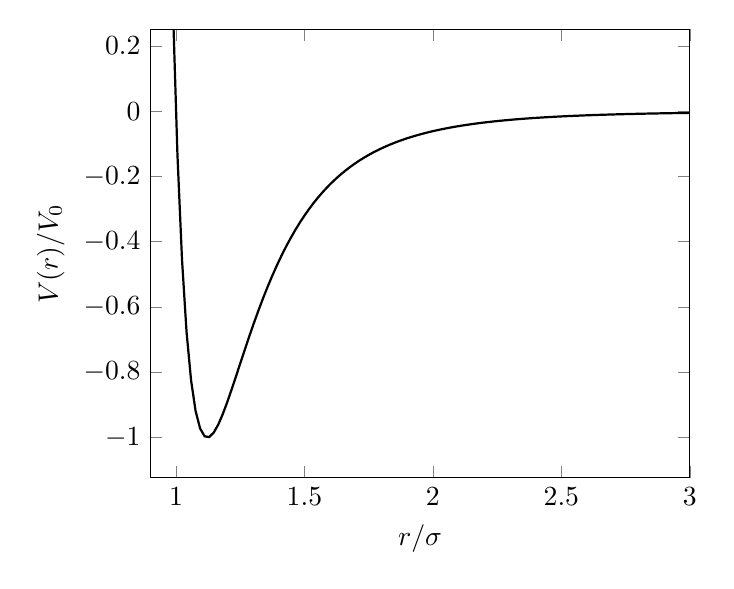
\begin{tikzpicture}
            \begin{axis}[xmin=0.9, xmax=3, ymax=0.25, xlabel={$r / \sigma$}, ylabel={$V(r) / V_0$}]
                \addplot[domain=0.9:3, samples=120, thick]{4*((1/x)^(12) - (1/x)^6)};
            \end{axis}
        \end{tikzpicture}
    \end{center}
\end{fquestion}

\begin{fquestion}{Was ist das Morse-Potential?}
    Das Morse-Potential
    $$V(r) = V_0 \left(1 - e^{-a (r - r_0)}\right)^2$$
    beschreibt die potentielle Energie eines zweiatomigen Moleküls.
    Es gilt näherungsweise am Ursprung $\exp (-a (r - r_0)) \approx 1 - a (r - r_0)$ und damit
    $$V(r) = V_0 a^2 (r - r_0)^2,$$
    was die Näherung des Morse-Potentials durch einen harmonischen Oszillator rechtfertigt.
    \begin{center}
        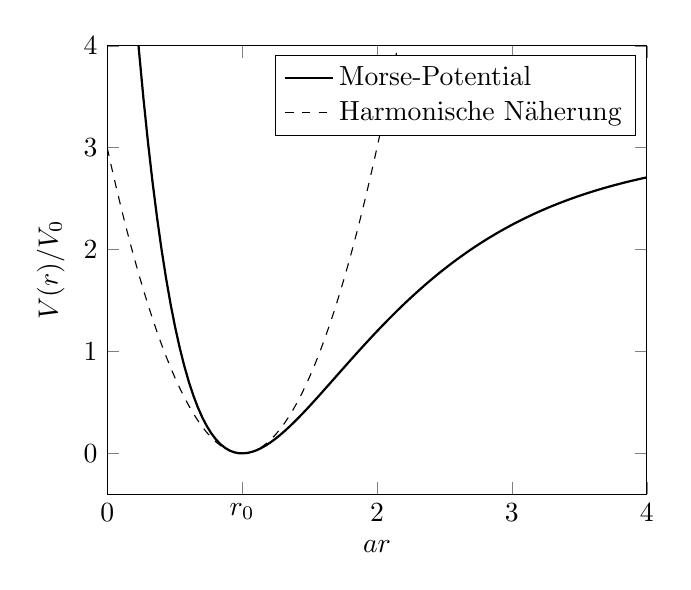
\begin{tikzpicture}
            \begin{axis}[xmin=0, xmax=4, ymax = 4, xlabel={$a r$}, ylabel={$V(r) / V_0$}, xtick={0,1,2,3,4},xticklabels={0, $r_0$, 2, 3, 4}, legend cell align={left}]
                \addplot[domain=0:4, samples=120, thick]{3*(1 - exp(-1 * (x - 1)))^2};
                \addlegendentry{Morse-Potential}
                
                \addplot[domain=0:4, samples=120, dashed] {3*1 * (x - 1)^2};
                \addlegendentry{Harmonische Näherung}
            \end{axis}
        \end{tikzpicture}
    \end{center}
\end{fquestion}

\begin{fquestion}{Wie sehen die Energieeigenwerte des Morse-Potentials aus?}
    Das Morsepotential hat die Eigenwerte
    $$E_n = \hbar \omega_0 \left(n + \frac{1}{2}\right) - \frac{\hbar^2 \omega_0^2}{4 V_0} \left(n + \frac{1}{2}\right)^2,$$
    wobei $\omega_0 = \frac{a}{2\pi} \sqrt{\frac{2 V_0}{m}}$.
    Der Abstand zweier Energieniveaus ist damit
    $$\Delta E = \hbar \omega_0 - \frac{\hbar^2 \omega_0^2}{2 V_0} (n + 1).$$
    Für kleine Quantenzahlen $n$ ist das Morse-Potential gut als hamonischer Oszillator genähert, dessen Energieniveaus für größer werdende $n$ zusammenrücken.
    
    In \autoref{tab:schwingungsparameter} sind beispielhafte Werte dargestellt
\end{fquestion}

\begin{fquestion}{Wie sieht das Morsepotential asymptotisch aus?}
    Es sieht exponentiell aus.
\end{fquestion}

\begin{fquestion}{Wie kann man ein Molekül anregen?}
    Die Photonenabsorption führt zu Vibrationen und Rotationen.
\end{fquestion}

\begin{table}[htb!]
    \centering
    \begin{tabular}{|c|c|ccc|ccc|}
        \hline
        & & \multicolumn{3}{c|}{Rotation $B$} & \multicolumn{3}{c|}{Vibration $\omega$} \\
        Molekül & $R / \si{pm}$ & $\si{cm^{-1}}$ & $\si{meV}$ & $\si{K}$ & $\si{cm^{-1}}$ & $\si{meV}$ & $\si{K}$ \\
        \hline
        $\text{H}_2$ & $74.16$ & $60.8$ & $7.24$ & $86.9$ & $4395$ & $523$ & $6278$ \\
        $\text{Li}_2$ & $267.3$ & $0.673$ & $0.08$ & $0.96$ & $351$ & $41.8$ & $501$ \\
        $\text{N}_2$ & $109.4$ & $2.010$ & $0.24$ & $2.87$ & $2359$ & $280$ & $3370$ \\
        $\text{O}_2$ & $120.7$ & $1.446$ & $0.17$ & $2.07$ & $1580$ & $188$ & $2257$ \\
        $\text{I}_2$ & $266.6$ & $0.037$ & $0.004$ & $0.05$ & $214$ & $25.5$ & $306$ \\
        \hline
        $\text{NO}$ & $115.1$ & $1.705$ & $0.203$ & $2.43$ & $1904$ & $227$ & $2720$ \\
        $\text{ICl}$ & $232.1$ & $0.114$ & $0.014$ & $0.16$ & $384$ & $45.71$ & $549$ \\
        $\text{HCl}$ & $127.1$ & $10.59$ & $1.26$ & $15.1$ & $2990$ & $356.0$ & $4271$ \\
        \hline
    \end{tabular}
    \caption{Gleichgewichtsabstände $R$ sowie Rotationskontansten $B$ und Vibrationsfrequenzen $\omega_0$ verschiedener Moleküle. }
    \label{tab:schwingungsparameter}
\end{table}

% \begin{question}{Wie sehen die Vibrationsniveaus aus?}
%     $10-100$ meV, welche Frequenzen sind das ???
%     Niveaus sind zunächst äquidistant, da Näherung als HO ???
%     makroskopische Betrachtung als Wärme, also Größenordnung von 300K == 25 meV
% \end{question}

\begin{fquestion}{Welche Ersetzungen muss man durchführen, um Rotationen zu beschreiben?}
    Bei der kinetischen Energie führt man die Ersetzung 
    $$\nabla \rightarrow J \text{ und } m \rightarrow I$$
    durch, wodurch dann $E_j = \frac{J^2}{2I} = \frac{\hbar^2 j (j + 1)}{2I}$.
    Der Abstand zweier Energieniveaus ist $\Delta E = \frac{\hbar^2}{I} (j + 1)$, wir nennen 
    $$B \equiv \frac{\hbar^2}{2 I} = \frac{\hbar^2}{2 \mu R^2}$$
    die Rotationskonstante eines Moleküls.
    Mit ihr ist $\Delta E = B (j + 1)$.
    
    In \autoref{tab:schwingungsparameter} sind beispielhafte Werte dargestellt, typischerweise liegen diese zwischen $\SI{1}{meV}$ und $\SI{10}{meV}$.
\end{fquestion}

% \begin{question}{Wie sehen die Rotationsniveaus aus?}
%      $0.1-1$ meV, welche Frequenzen sind das ???
%      Niveaus sind äquidistant, für höhere Energien leichte Verringerung wegen Änderung des Trägheitsmoments ???
% \end{question}

\begin{fquestion}{Was regt ein Mikrowellenherd an?}
    Rotationen
\end{fquestion}

\begin{fquestion}{Durch welches Potential lässt sich die Bindung des $H_2^+$-Ion beschreiben?}
    Zum Analysieren des $H_2^+$-Molekülions verwendet man die LCAO-Methode.
    Man macht entsprechend den Ansatz
    $$\ket{\psi_\pm} = C_\pm (\ket{\phi_1} \pm \ket{\phi_2}),$$
    wobei $\ket{\phi_1}$ und $\ket{\phi_2}$ die Grundzustandswellenfunktionen des Wasserstoffs um Proton $1$ und $2$ sind.
    Die Normalisierungskonstante ist hier $C_\pm = \left(2 (1 \pm S)\right)^{-1 / 2}$ mit dem Überlappintegral $S = \braket{\psi_1}{\psi_2}$.
    
    Die Energien erhält man schlussendlich aus dem Hamiltonian 
    $$H = \frac{-\nabla^2}{2m} + \frac{e^2}{4 \pi \varepsilon_0} \left(-\frac{1}{r_1} - \frac{1}{r_2} + \frac{1}{R}\right)$$
    über 
    $$E_\pm(R) = \bra{\psi_\pm} H \ket{\psi_\pm} = \frac{H_S \pm H_A}{1 \pm S}$$
    mit dem symmetrischen Energieanteil $H_S = \bra{\phi_1} H \ket{\phi_1} = \bra{\phi_2} H \ket{\phi_2}$ sowie dem antisymmetrischen Anteil $H_A = \bra{\phi_1} H \ket{\phi_2}$.
\end{fquestion}

\begin{fquestion}{Wie sieht dann die Lösung aus?}
    Numerisch kann man diese mit dem Coulomb-Integral $C = \bra{\phi_1} \frac{1}{r_2} \ket{\phi_1} + \frac{1}{R}$ und dem Austausch-Integral $K = \bra{\phi_1} \frac{1}{r_2} \ket{\phi_2} + \frac{S}{R}$ zu
    $$E_\pm = -E_0 \pm \frac{J \pm K}{1 \pm S}$$
    ermitteln.
    
    Ist das Elektron bei beiden Protonen in der $1\mathrm{s}$-Schale ($\phi_1(r_1) = \phi_2(r_2) = \sqrt{\frac{1}{a_0^3 \pi}} \exp\left(-\frac{r_{1,2}}{a_0}\right)$) so folgt
    $$\begin{aligned}
        S(R) &= e^{-R} \left(1 + R + \frac{1}{3} R^2\right) \\
        J(R) &= e^{-2R} \left(1 + \frac{1}{R}\right) \\
        K(R) &= e^{-R} \left(\frac{1}{R} - \frac{2}{3} R \right)
    \end{aligned} $$
    
    \begin{center}
        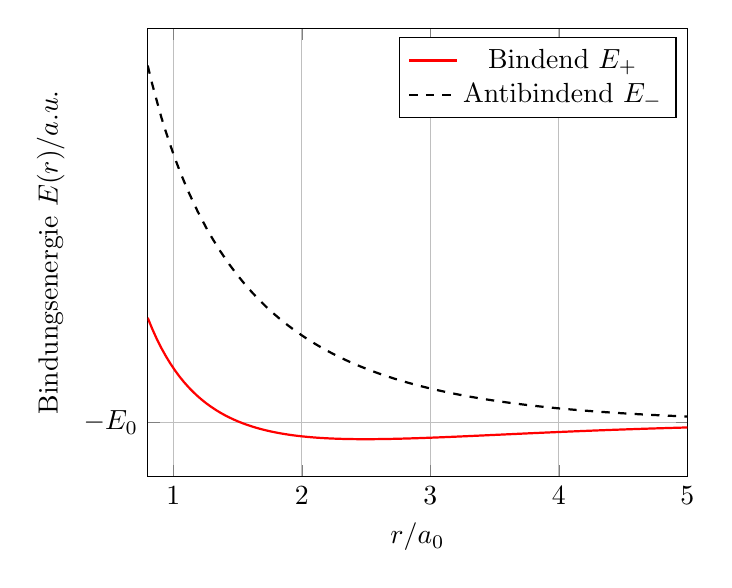
\begin{tikzpicture}[
        declare function={ 
                S(\x) = exp(-\x) * (1 + \x + 1/3 * \x^2);
                J(\x) = exp(-2*\x) * (1 + 1/\x);
                K(\x) = exp(-\x) * (1/\x - 2/3 * \x);
                Ep(\x) = (J(\x) + K(\x)) / (1 + S(\x));
                Em(\x) = (J(\x) - K(\x)) / (1 - S(\x));
            },
        ]
            \begin{axis}[xmin=0.8, xmax=5, xlabel={$r / a_0$}, ylabel={Bindungsenergie $E(r) / \si{a.u.}$},ytick={0}, yticklabels={$-E_0$}, grid=both]
                \addplot[domain=0.8:5, samples=120, thick, red]{Ep(x)};
            	\addlegendentry{Bindend $E_+$}

                \addplot[domain=0.8:5, samples=120, thick, dashed]{Em(x)};
            	\addlegendentry{Antibindend $E_-$}
            \end{axis}
        \end{tikzpicture}
    \end{center}
\end{fquestion}

\begin{fquestion}{Welchen Bindungszustand nimmt das $H_2^+$-Molekül ein?}
    Den symmetrischen, bei dem das  Elektron die größte Aufenthaltswahrscheinlichkeit zwischen den Protonen hat.
\end{fquestion}

\begin{fquestion}{Wie sind die Größenordnungen des $H_2^+$-Potentials?}
    Mit der oben beschriebenen Methode erhält man eine Bindungsenergie von ungefähr $\SI{-1.76}{eV}$ bei einem Gleichgewichtsabstand von $\SI{1.3}{\angstrom}$.
    
    Experimentell erhält man $E = \SI{-2.8}{eV}$ und $R = \SI{1.06}{\angstrom}$.
\end{fquestion}

\begin{figure}[tb!]
    \centering
    \subcaptionbox{Schematische Darstellung der Intensitätsverteilung von vibronischen Übergängen gemäß dem Franck-Condon-Prinzip. Die Zahlen $\nu'' \rightarrow \nu'$ geben dabei den Anfangszustand $\nu''$ und Endzustand $\nu'$ der Vibration an. \label{subfig:franck_condon:1}}[0.49\linewidth]{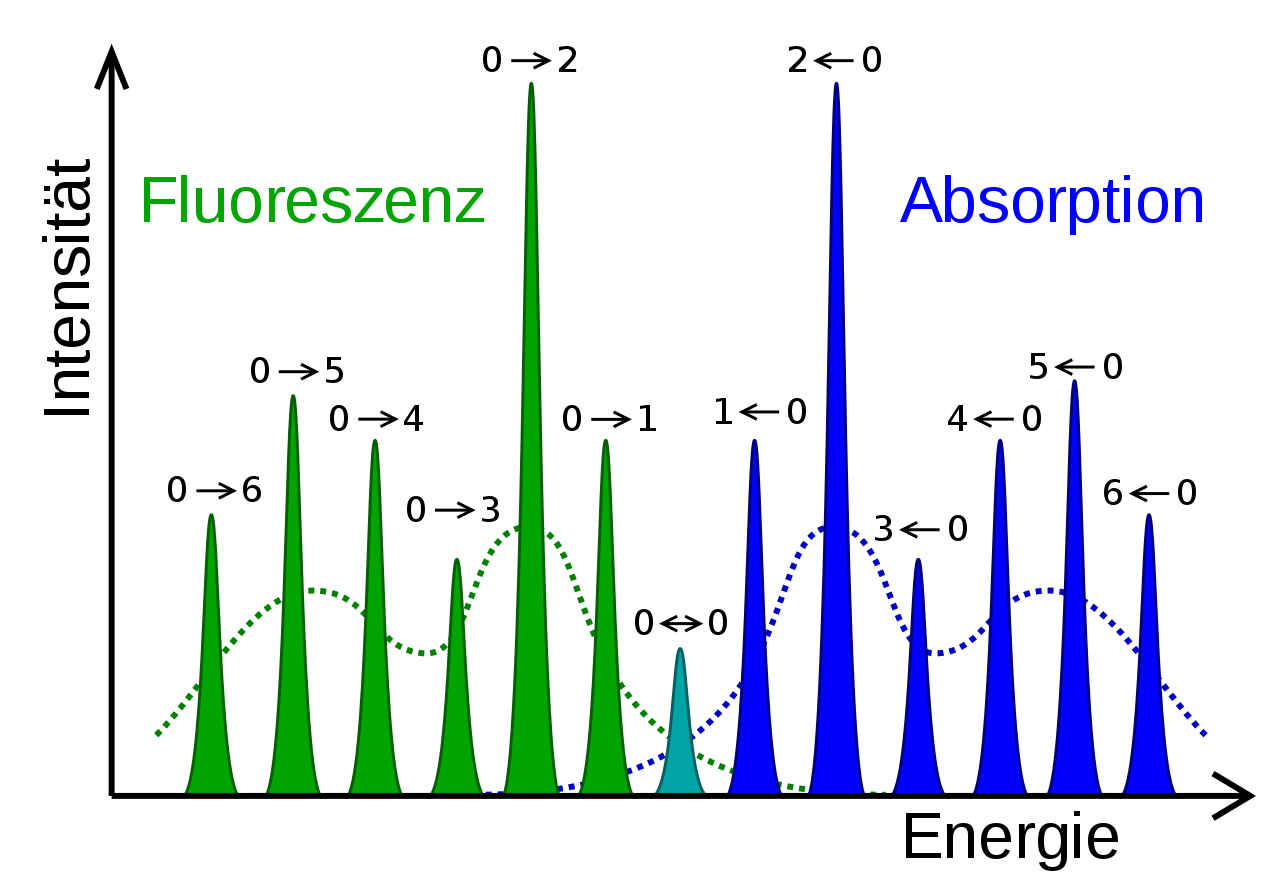
\includegraphics[width=\linewidth]{img/1280px-Franck-Condon-Prinzip_Intensitaeten.svg.png}}
    \subcaptionbox{Energie eines zweiatomigen Moleküls in Abhängigkeit vom theoretisch festgehaltenen Abstand der Kerne, für zwei verschiedene Zustände der Elektronenhülle (schematisch). Die Schwingungszustände sind mit ihren Wellenfunktionen für den Kernabstand auf der Höhe der jeweiligen Energie eingezeichnet. Die beiden Pfeile stellen vibronische Übergänge dar. \label{subfig:franck_condon:2}}[0.49\linewidth]{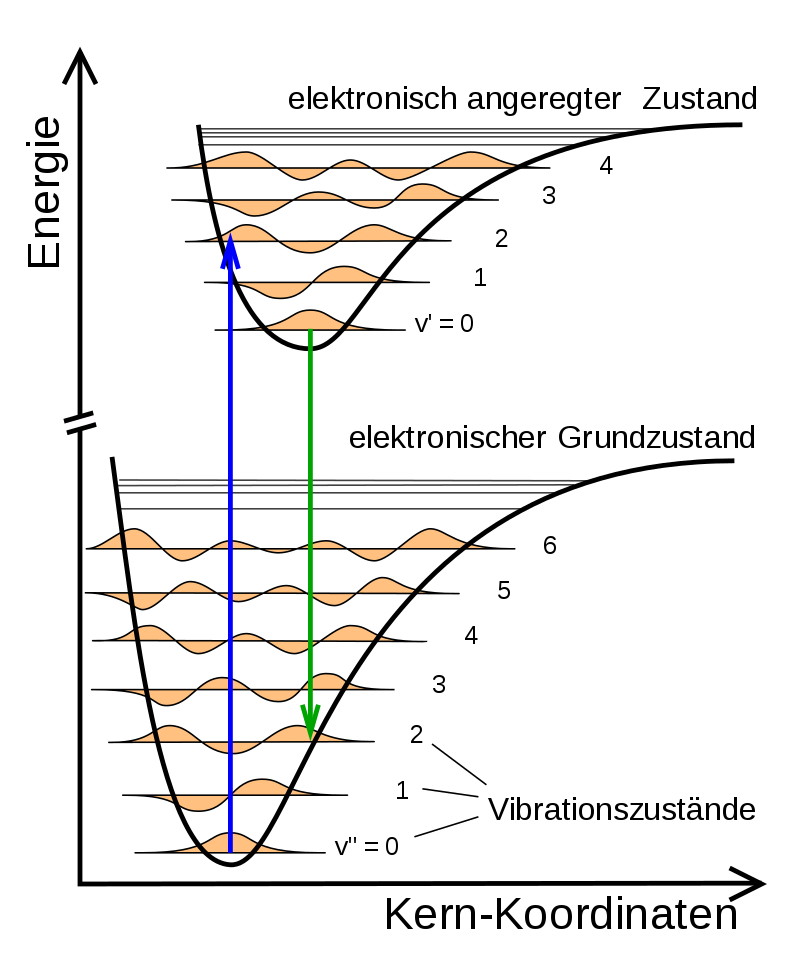
\includegraphics[width=\linewidth]{img/800px-Franck-Condon-Prinzip.svg.png}}
    \caption{Abbildungen zum Franck-Condon-Prinzip. \refimgsource{Wikimedia}{https://de.wikipedia.org/wiki/Franck-Condon-Prinzip}{23.02.2022}{public domain}}
    \label{fig:franck_condon}
\end{figure}

\begin{fquestion}{Was ist das Frank-Condon-Prinzip?}
    Das Frank-Condon-Prinzip beschreibt das Verhalten von Vibrationseigenzuständen eines Moleküls bei einer Änderung des Zustands des Elektrons (dem Übergang in eine andere Schale).
    Wegen seiner hohen Masse ist die Schwingungsperiode des Kerns mit $\approx \SI{e-13}{s}$ sehr viel länger als die Dauer eines elektrischen Übergangs $\approx \SI{e-15}{s}$; die Kernkonfiguration bleibt beim Übergang also starr (Born-Oppenheimer-Näherung).
    
    Dadurch geht der Vibrationszustand bevorzugt in einen anderer Quantenzahl, aber großer Überlappung über.
    Der neue Vibrationszustand ist dementsprechend nicht mehr der Vibrationsgrunzustand.
    Siehe \autoref{fig:franck_condon} für eine Illustration, besonders der blaue Pfeil für die Anregung.
\end{fquestion}

\begin{fquestion}{Wie steht das Frank-Condon-Prinzip mit dem Stokes-Shift im Zusammenhang?}
    Der Stokes-Shift beschreibt eine Verschiebung der Wellenlänge von Licht zwischen Absorption und Emission, etwa bei der Fluoreszenz:
    \begin{center}
        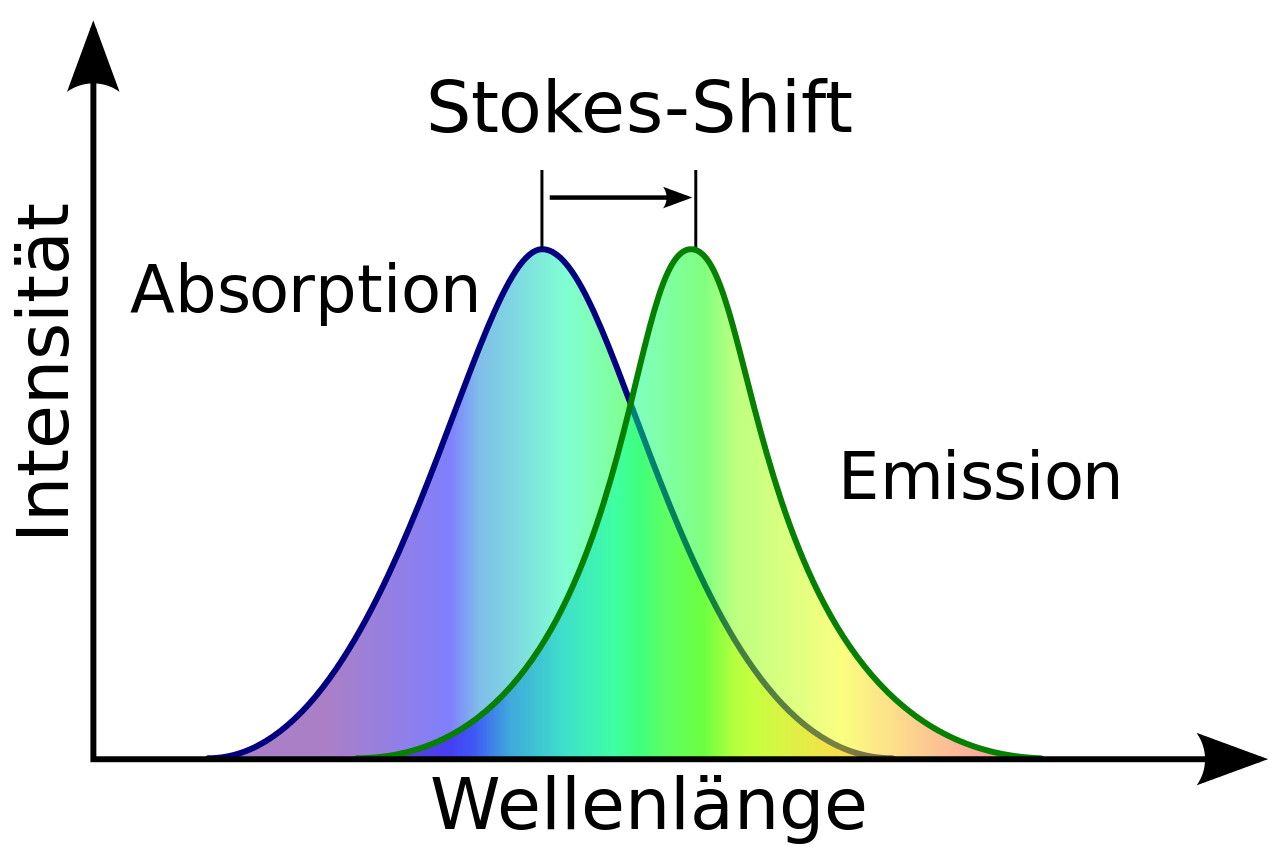
\includegraphics[width=0.4\linewidth]{img/1280px-Stokes-Verschiebung.svg.png}
    \end{center}
    Er entsteht dabei dadurch, dass ein Molekül nach der Anregung nicht mehr im vibratonischen Grundzustand ist (Franck-Condon-Prinzip).
    Die Abregung des vibratonischen Zustandes ist der elektronischen Abregung gegenüber bevorzugt, entsprechend findet zunächst die Abregung in den Grundzustand der Vibrationsmoden statt.
    Danach erfolgt erst die elektrische Abregung, welche entsprechend mit weniger Energie (höherer Wellenlänge) stattfindet.
    In \autoref{subfig:franck_condon:2} ist dies durch den blauen Pfeil für die elektrische Anregung in den grünen Pfeil für die elektrische Abregung dargestellt.
\end{fquestion}

% \begin{question}{Wie kommt die Bindung zustande?}
%     LCAO (Linear combination of atomic orbitals)
%     kovalente Bindung ???
% \end{question}

% \begin{question}{Ist das immer so?}
%     nein, kommt auf das Potential an
% \end{question}

\begin{fquestion}{Wenn man den antibindenden Zustand im Wasserstoff-Molekül zu Helium zusammenschiebt, was hat man dann?}
    Der antibindende Wasserstoffzustand hat näherungsweise die Form eines Heliums ${}_{2}\text{H}^+$ im $2p$-Zustand:
    \begin{center}
        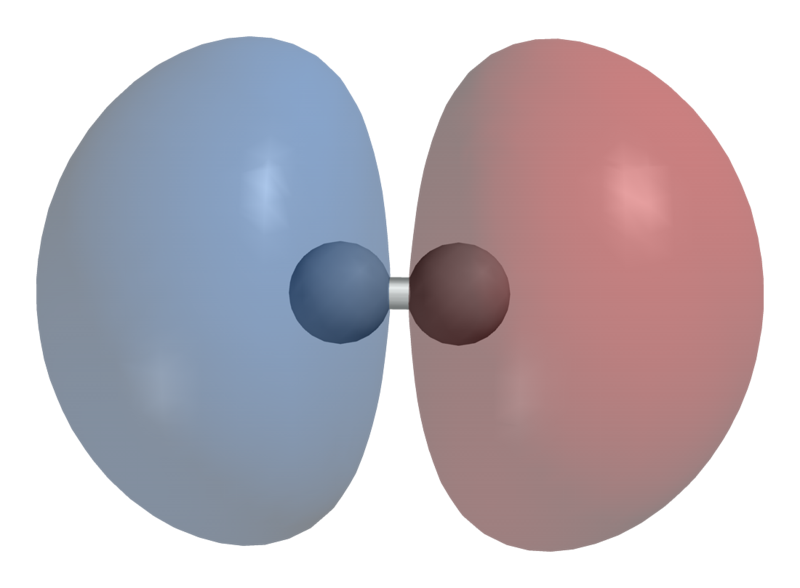
\includegraphics[width=0.3\linewidth]{img/800px-Dihydrogen-LUMO-phase-3D-balls.png}
    \end{center}
    \refimgsource{Wikimedia}{https://commons.wikimedia.org/wiki/File:Dihydrogen-LUMO-phase-3D-balls.png}{22.02.2022}{public domain}
\end{fquestion}

% \begin{question}{Spaltet der Grundzustand symmetrisch auf oder nicht bzgl der Energie?}
%     eigentlich ja, aber wegen der Absenkung der kinetischen Energie nicht ganz
% \end{question}

\begin{fquestion}{Wie sieht die Wellenfunktion eines Moleküls asymptotisch aus?}
    % Wie gewohnt exponentiell, übliches Verhalten für $\frac{1}{r^n}$-Potentiale.
    Exponentiell, wie für gebundene Zustände allgemein üblich.
\end{fquestion}

% \begin{question}{Beim Yukawa-Potential des Deuterons war die Pion-Masse relevant. Welche hier?}
%     Elektron für Bindung verantwortlich, also die Elektronenmasse.
% \end{question}

\subsection{Umrechnungen}

$\hbar c \simeq \SI{200}{MeV\,fm}$, $\SI{1}{meV} \simeq \SI{12}{K} \simeq \SI{8.4}{cm^{-1}}$ (Achtung: lineare Wellenzahl, siehe \autoref{fig:harmonic wave properties conversion}).
\\
Energie in Frequenz: $\SI{1}{eV} = \frac{e}{h} = f = \SI{242}{THz}$ (Achtung: $f\neq \omega = 2\pi f$).

\begin{figure}[!ht]
    \centering
    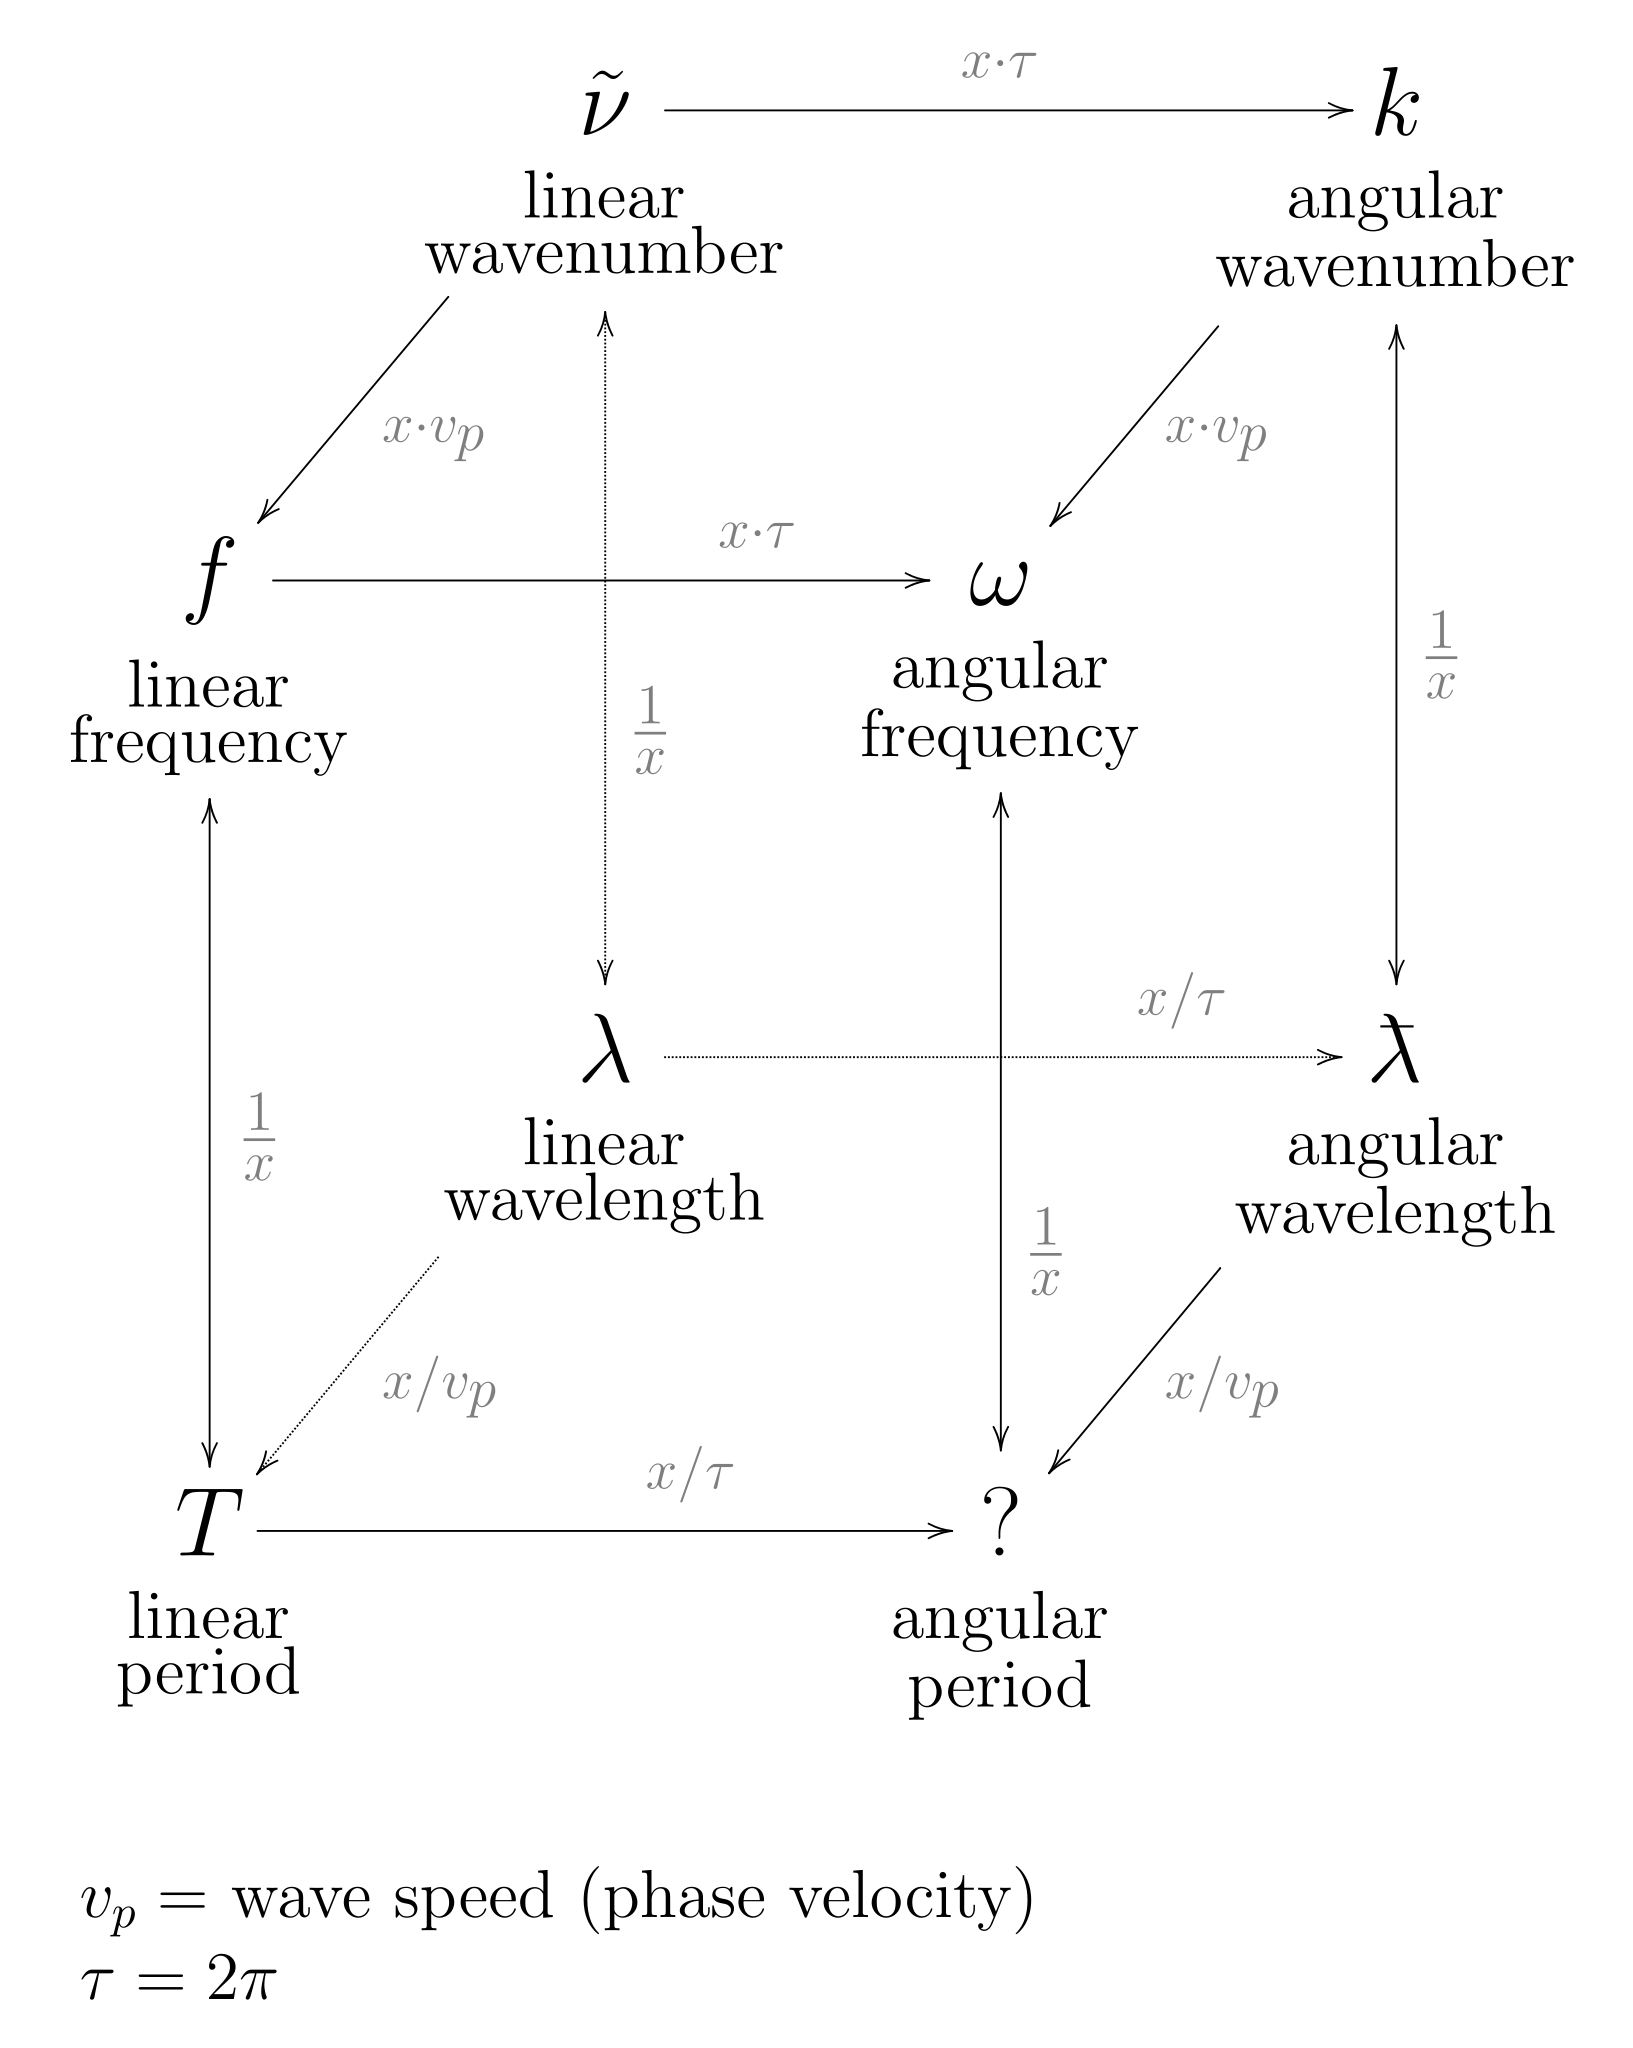
\includegraphics[width=.8\linewidth]{img/Commutative_diagram_of_harmonic_wave_properties.png}
    \caption{Grafische Darstellung der verschiedenen Eigenschaften einer Welle mit entsprechenden Konvertierungen.
    \refimgsource{Wikimedia}{https://commons.wikimedia.org/wiki/File:Commutative\_diagram\_of\_harmonic\_wave\_properties.svg}{24.02.2022}{public domain}}
    \label{fig:harmonic wave properties conversion}
\end{figure}




